In this study, different types of systematic uncertainty are taken into account. The distribution of $\ntrk$ and BDT for truth-labelled quark-/gluon-jets are given by the MC simulation samples, therefore, theoretical uncertainties originate from aspects encompassing the modelling of the MC simulation, such as choices involving parton showering, hadronisation, matrix element, PDFs, scale variations, and Splitting-Kernel effects. Furthermore, experimental uncertainties such as JES and JER, tracking reconstruction efficiencies are meticulously incorporated. The potential impact of methodological choices, including \ntrk~or BDT re-weighting, as well as the non-closure behaviour of MC simulations, is propagated to the resultant SFs.

The nominal result in this analysis is provided using \pythia8 MC samples, all other MC samples are considered as alternative samples to study corresponding systematic uncertainty.


\subsubsection{Parton shower modelling uncertainty}
    The different chose of algorithmic or parametric in the modelling of the parton shower could result in different SF result. This systematic uncertainty is estimated by comparing the SFs extracted from two MC samples with the same ME and hadronisation but different types of showers: \herwig Angular-ordered and \herwig Dipole samples. The corresponding fractions of quarks and gluons present in these two MC samples, are presented in Figure~\ref{fig:QG-herang-Frac}. The difference of extracted SFs between these two samples is less than 10\% for quark signal efficiency and around 20\% for gluon rejection efficiency. While the influence on quark scale factors is negligible, it takes on a dominant role in the context of gluon scale factors.
    \begin{figure}[htb]
    	\centering
    	\subfloat[\herwig Angular]{\label{fig:QG-herang-Fmc}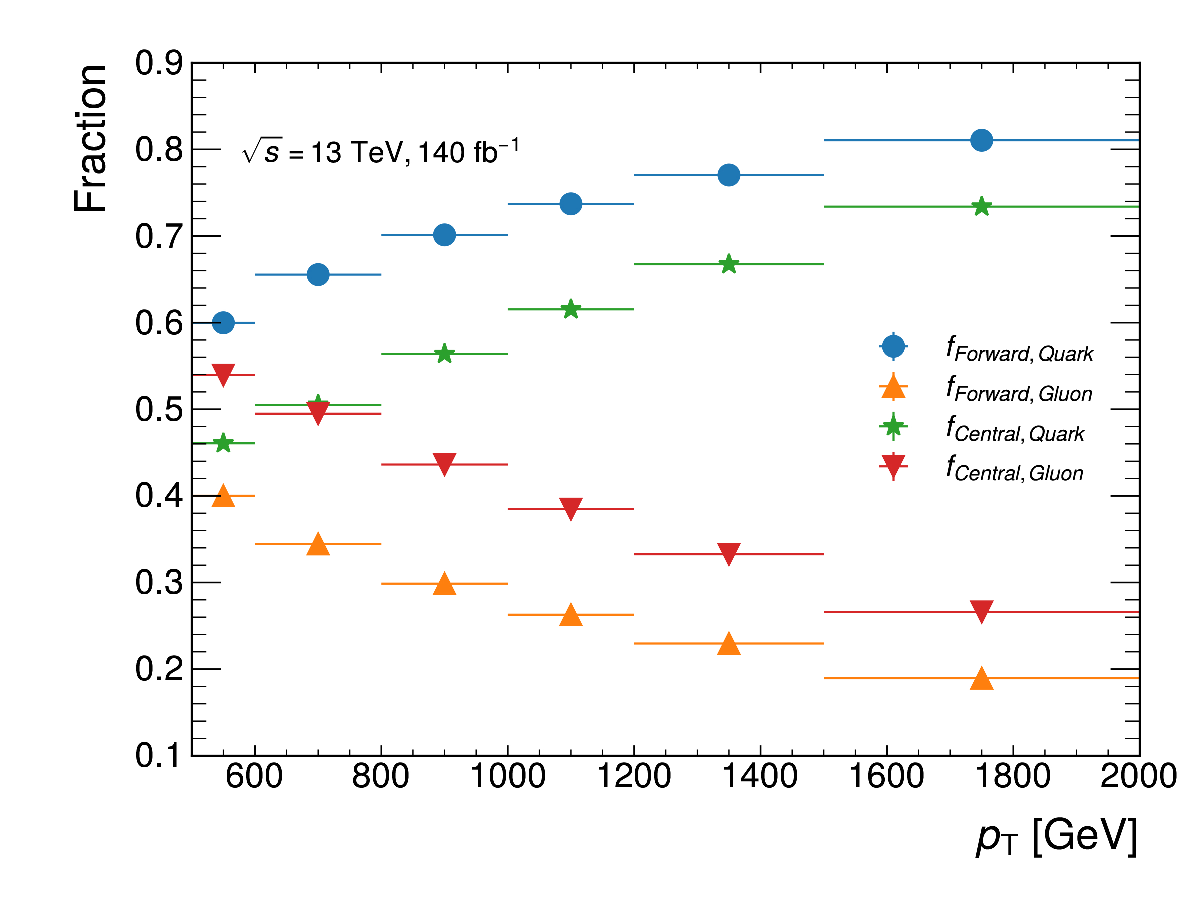
\includegraphics[width=0.45\textwidth]{fig/parton_shower/herwigangle/plots/ADE/Fractions/none_event_weight/Fraction.pdf}} \quad
    	\subfloat[\herwig Dipole]{\label{fig:QG-herdip-Fmc}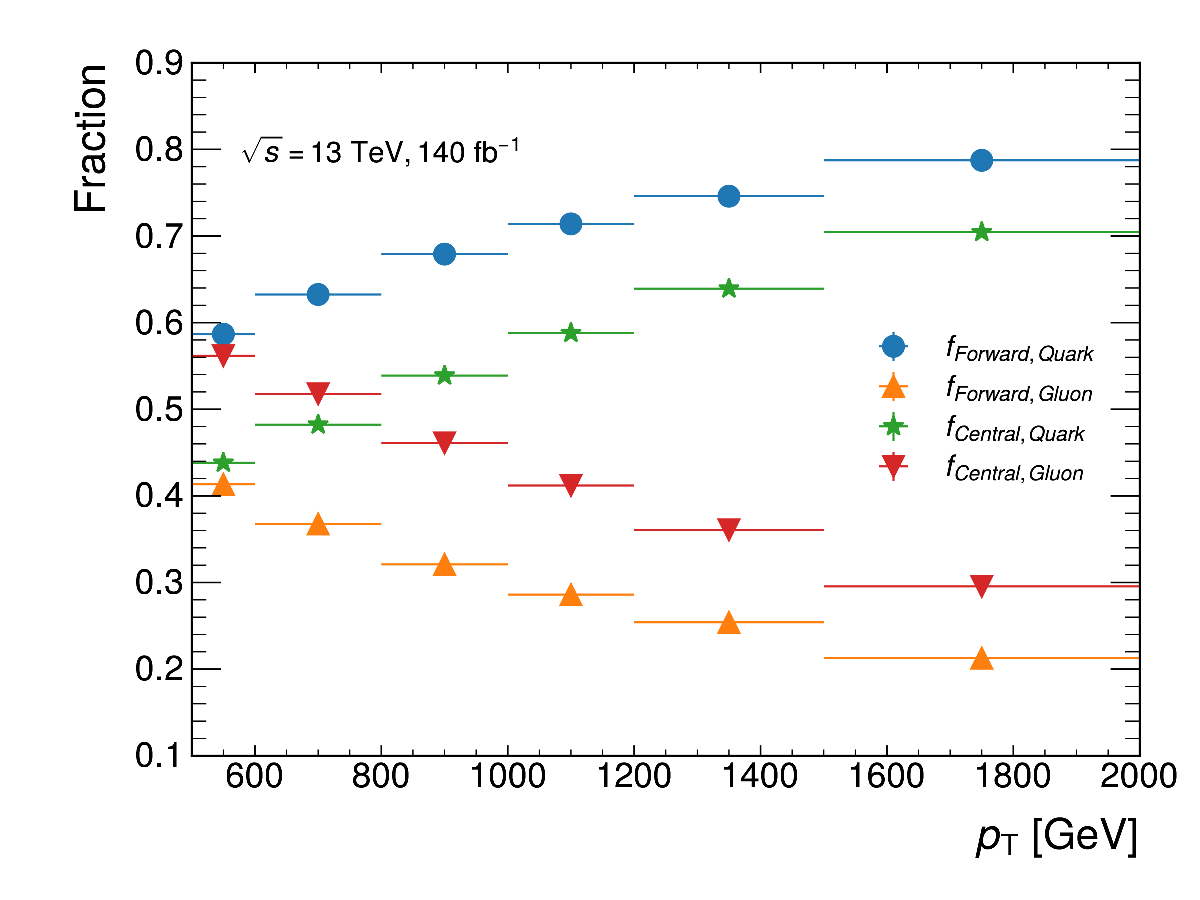
\includegraphics[width=0.45\textwidth]{fig/parton_shower/herwigdipole/plots/ADE/Fractions/none_event_weight/Fraction.pdf}}
    	\caption[]{
    		Fractions of quark- gluon-jets of \herwig angular \subref{fig:QG-herang-Fmc} and  \herwig dipole \subref{fig:QG-herdip-Fmc} samples.
    		%.
    		\label{fig:QG-herang-Frac}
    	}
    \end{figure}

    
\FloatBarrier
\subsubsection{Hadronisation modelling uncertainty}
    The uncertainty from hadronisation modelling is given by the difference between the extracted SFs from the \sherpa MC samples with cluster-based hadronisation modelling and string-based hadronisation modelling, separately. The corresponding fractions of quarks and gluons present in these two MC samples are presented in Figure~\ref{fig:QG-had-Frac}. The uncertainty on the SFs range from 1\% to 8\% for both jet types.
    
    \begin{figure}[htb]
    	\centering
    	\subfloat[\sherpa String-based]{\label{fig:QG-had-Fmc}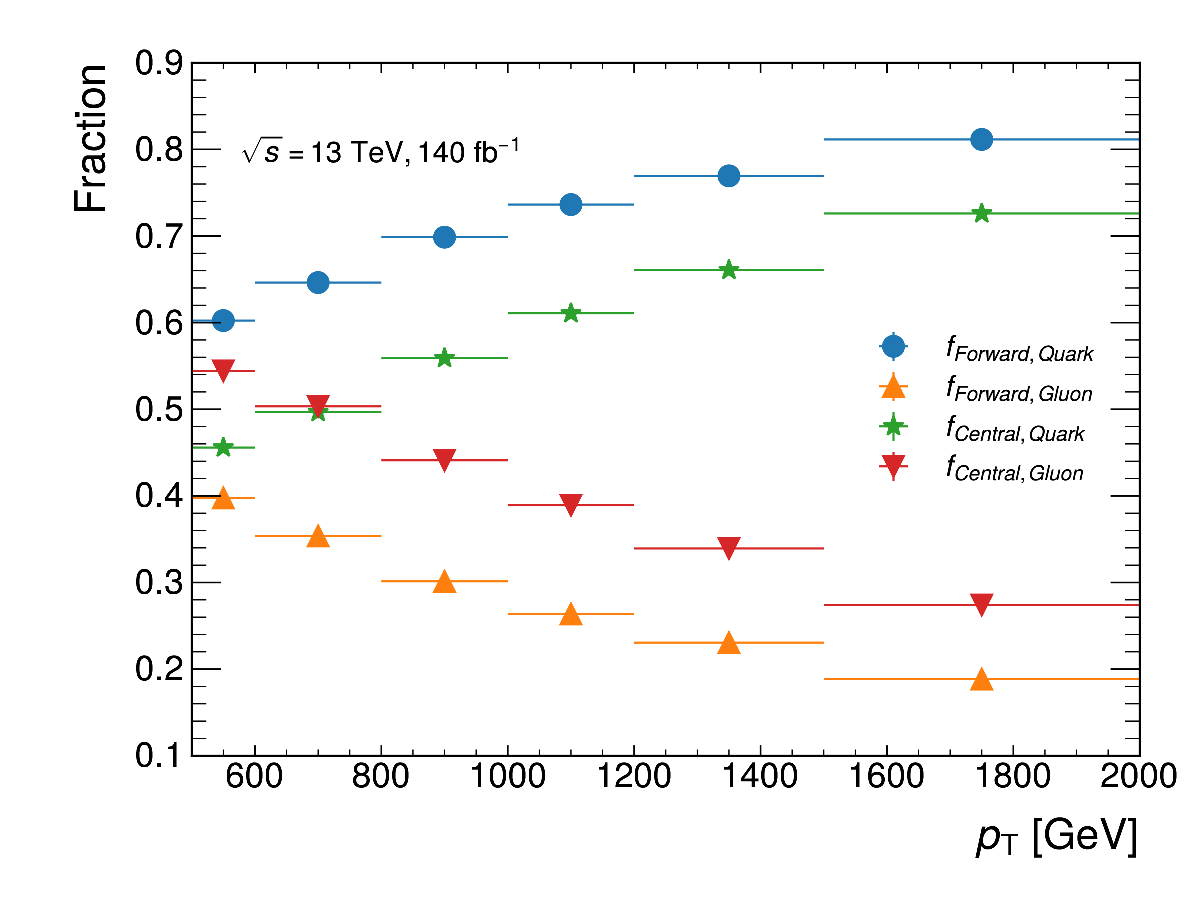
\includegraphics[width=0.45\textwidth]{fig/hadronization/sherpalund/plots/ADE/Fractions/none_event_weight/Fraction.pdf}} \quad
    	\subfloat[\sherpa Cluster-based]{\label{fig:QG-lund-Fmc}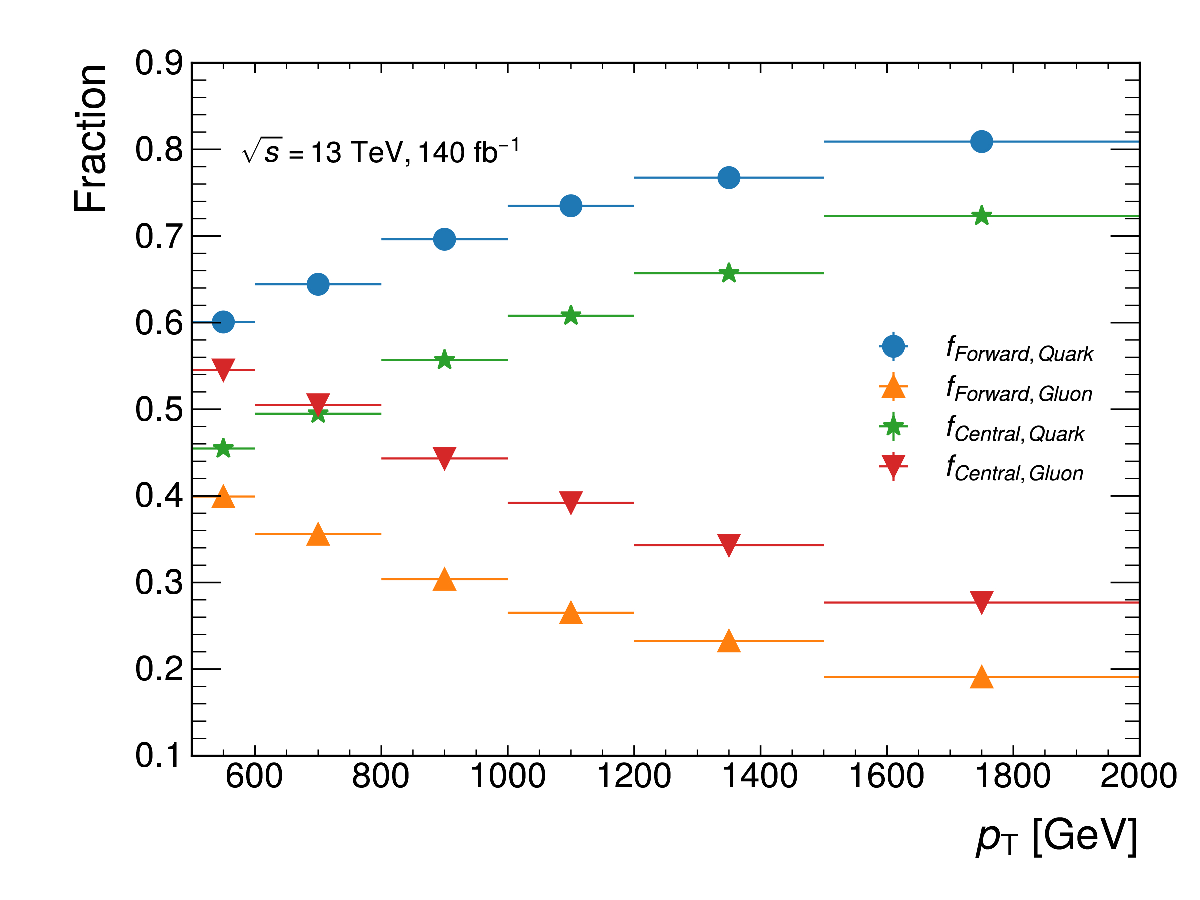
\includegraphics[width=0.45\textwidth]{fig/hadronization/sherpa/plots/ADE/Fractions/none_event_weight/Fraction.pdf}} 
    	\caption[]{
    		Fractions of quark- and gluon-jets in each \sherpa sample. %
    		%.
    		\label{fig:QG-had-Frac}
    	}
    \end{figure}

\FloatBarrier

\subsubsection{Matrix element uncertainty}

The  uncertainty introduced by different types of ME in the MC samples is taken from the differences in the extracted SFs in two MC samples with different ME : \powheg and \pythia. The corresponding fractions of quarks and gluons present in the \powheg samples are presented in Figure~\ref{fig:QG-pow-Frac}. 


\begin{figure}[htb]
	\centering
	\label{fig:QG-pow-Fmc}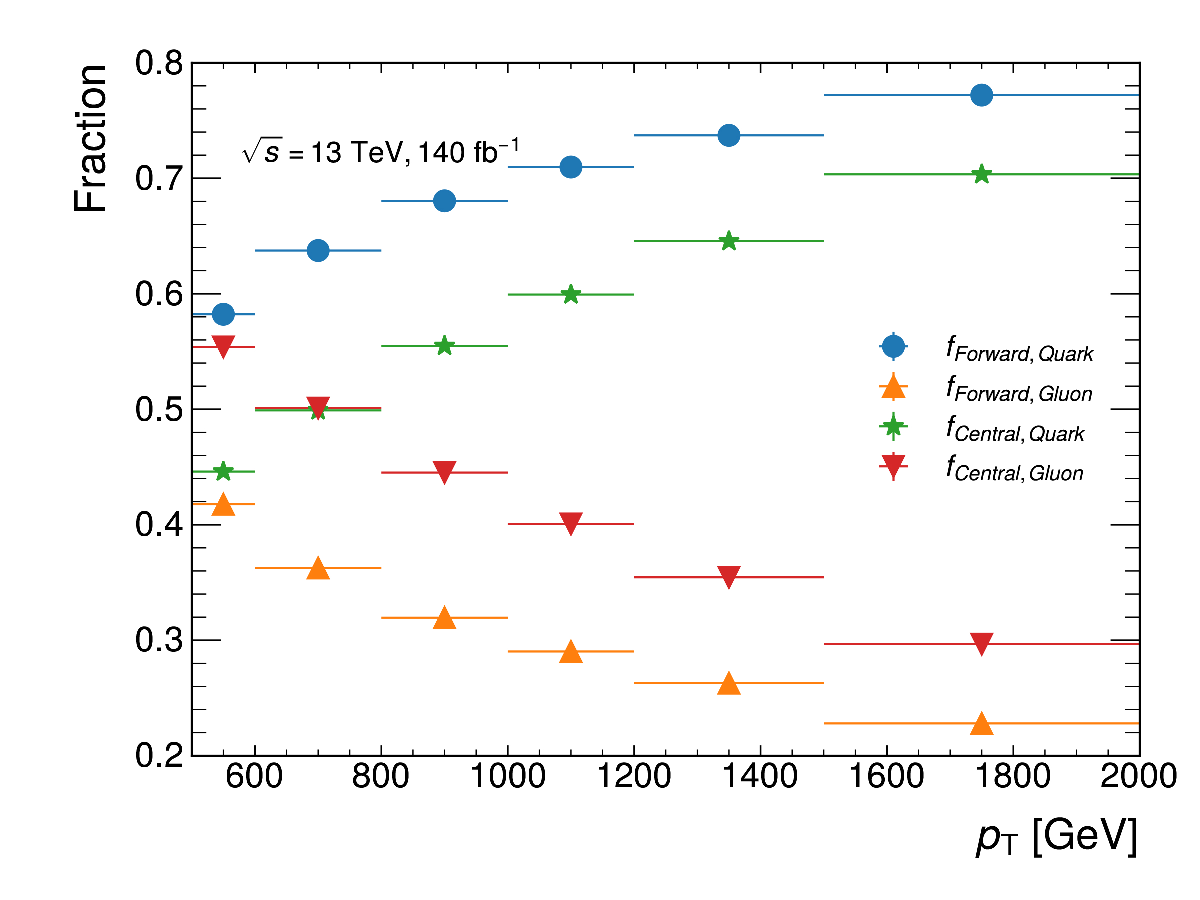
\includegraphics[width=0.45\textwidth]{fig/powhegpythia/plots/ADE/Fractions/none_event_weight/Fraction.pdf}
	\caption[]{
		Fractions of quark jets and gluon jets in \powheg samples. %
		%.
		\label{fig:QG-pow-Frac}
	}
\end{figure}

\FloatBarrier
    \subsubsection{PDF uncertainty}
  The uncertainty from the PDF set is evaluated using \textsc{LHAPDF}~\cite{LHAPDF} package which provides the PDF internal variations for each PDF set, a \nnpdftwo~set is chosen to evaluate the various weights which depend on the momentum fraction. The PDF uncertainty is given by changing the nominal PDF weight to the systematic variation, then compare the SFs extracted from each of variations. The PDF uncertainty is around 5\% - 7\% level and almost negligible compared to others.

  
    \subsubsection{Scale variation uncertainty}
  The variation of the renormalisation $(\mu_R)$ and factorisation $(\mu_F)$ scales in QCD is used to evaluate the uncertainty caused by missing higher order corrections. The nominal \pythia sample is used for such estimation. In total there are 7 scale variations
  $(\mu_R, \mu_F)$ in (2,2), (2,1), (1,1), (1,2), (1,0.5), (0.5,1), (0.5,0.5) studied in this analysis. The scale uncertainty is given by taking the maximum shift of the envelope with respect to the nominal one at each working points. The total scale uncertainty is around 4\% - 7\%. 

\subsubsection{Splitting-Kernel variation uncertainty}
All formulations of shower processes are constructed on the fundamental foundation of the universal behaviour exhibited by singular infrared (soft and/or collinear) limits within QCD. Nonetheless, when one ventures beyond these limits into the physical phase space where these kernels are employed as approximations, there are in principle infinitely many different radiation functions to choose from, sharing the same singular terms but having different non-singular ones.  The Splitting-Kernel variations~\cite{Mrenna:2016sih} are variations of the non singular part of the splitting functions, for initial-state radiation and final-state radiation. Such uncertainty is less than 1\%.
  
    \subsubsection{Tracking uncertainty}

he number of associated tracks is the most important input for both taggers, with tracking-related systematics exerting an impact on the measurement of SFs. he uncertainty associated with reconstructed tracks is partitioned into two components: the uncertainty pertaining to track reconstruction efficiency and the MC fake rate~\cite{ATLAS:2017kyn}. Both sources of uncertainty are factored in to recalibrate the count of tracks associated with jets.

 The track reconstruction efficiency uncertainty originates from material-related uncertainties, which constitutes the prevailing source, as well as from considerations related to the physics model. These uncertainties are estimated through a comparison of track efficiency across samples that encompass diverse detector modelling configurations. On the other hand, the MC fake rate is determined by contrasting the trends in a specific aspect of track multiplicity as a function of the average number of interactions per bunch crossing between empirical data and the MC simulation.The disparity in final SFs between the nominal value and the outcome of the systematic variation contributes to the tracking systematic uncertainty. This uncertainty spans a range of approximately 1\% to 8\%.

  \subsubsection{JES /JER uncertainty }
The uncertainties associated with JES stem from the process of calibrating the transverse momentum balance between jets located in the central and forward regions, while also accommodating uncertainties linked to single-particle and test beam measurements. The JER uncertainties encompass the disparities between data and the MC. For each JES/JER variation, a corresponding SF is derived, and the difference between the nominal value and the variation is computed to determine the systematic uncertainty. The cumulative JES/JER uncertainty amounts to approximately 0.2\%.
  
    \subsubsection{{\ntrk} / BDT re-weighting}
  The quark-enriched and gluon-enriched regions are defined by comparing the $\eta$ of leading and subleading jets, introduces to an $\eta$ dependency from track reconstruction process. A re-weighting factor defined by Equation~\ref{eq:QG-reweight} is applied on {\ntrk} and BDT taggers for each event to reduce the impact from different track multiplicity in different $\eta$ range. The re-weighting factors acquired from truth-labelled gluon jets are regarded as an alternative source of contribution to the systematic uncertainty. It's worth noting that the differences arising from the re-weighting procedure remain comparatively minor (about 0.1\% - 0.5\%) in comparison to other sources of uncertainty.
  
  
  The distributions of \ntrk~and BDT for extracted quark and gluon-jets after re-weighting with quark factor have been shown in the previous chapter. The truth distribution of quark/gluon in forward/central jets using gluon factors are shown in Figure~\ref{fig:QG-pythia-NtrkMCExtracted-Reweight-Compare1_g} for \ntrk~and Figure~\ref{fig:QG-pythia-GBDTMCExtracted-Reweight-Compare1_g} for BDT, respectively.  Figure~\ref{fig:QG-pythia-NtrkData500Gluon},  Figure~\ref{fig:QG-pythia-NtrkData800Gluon} shows the distributions of extracted quark and gluon-jets after reweighting with gluon factor.
  
  
  
  
  \begin{figure}[htb]
  	\centering
  	\subfloat[ ]{\label{fig:QG-pythia-NtrkMCExtractedGluonFactor-500-600-Ntrk}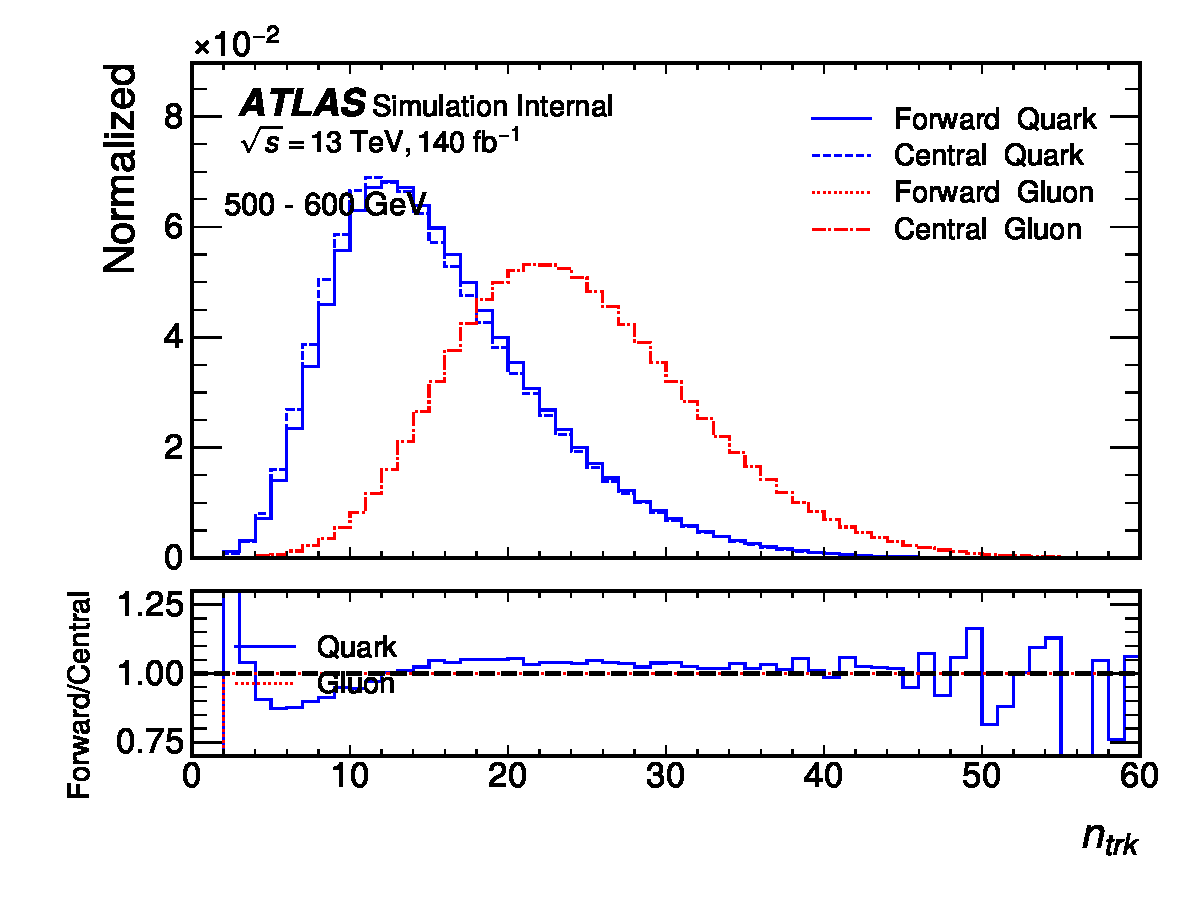
\includegraphics[width=0.45\textwidth]{fig/gluon_reweight/plots/ADE/FvsC/jet_nTracks_quark_reweighting_weights/jet_nTracks/MC_truth_Q_G_FvsC_500_jet_nTracks_quark_reweighting_weights.pdf}} \quad
  	\subfloat[$Jets :800<\pt<1000\GeV$~(\pythia8) ]{\label{fig:QG-pythia-NtrkMCExtractedGluonFactor-800-1000-Ntrk}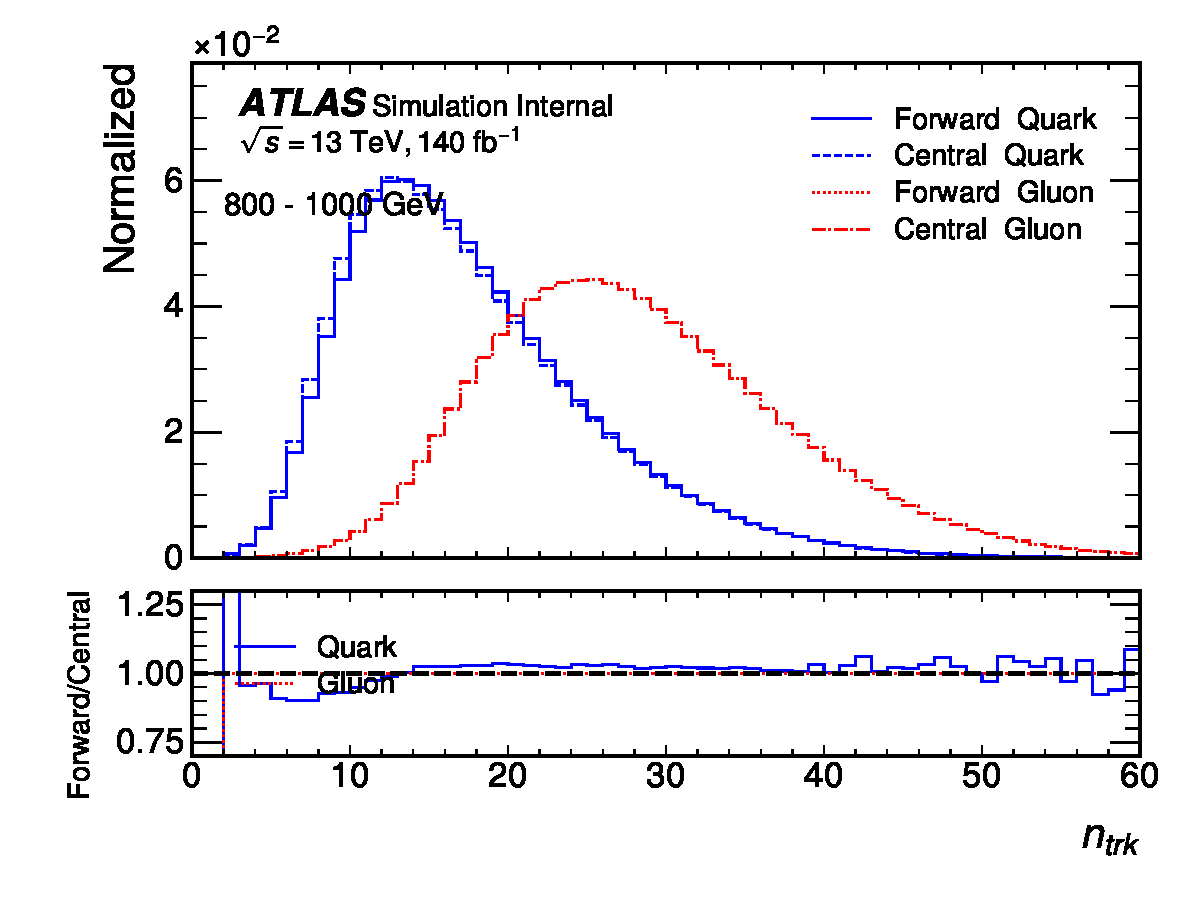
\includegraphics[width=0.45\textwidth]{fig/gluon_reweight/plots/ADE/FvsC/jet_nTracks_quark_reweighting_weights/jet_nTracks/MC_truth_Q_G_FvsC_800_jet_nTracks_quark_reweighting_weights.pdf}}
  	\caption[]{
  		The distribution of {\ntrk} for jets between 500-600 GeV  \subref{fig:QG-pythia-NtrkMCExtractedGluonFactor-500-600-Ntrk} and 800-1000 GeV  \subref{fig:QG-pythia-NtrkMCExtractedGluonFactor-800-1000-Ntrk} after {\ntrk} re-weighting using gluon factor. 
  		\label{fig:QG-pythia-NtrkMCExtracted-Reweight-Compare1_g}
  	}
  \end{figure}
  
  \begin{figure}[htb]
  	\centering
  	\subfloat[ ]{\label{fig:QG-pythia-GBDTMCExtractedGluonFactor-500-600-Ntrk}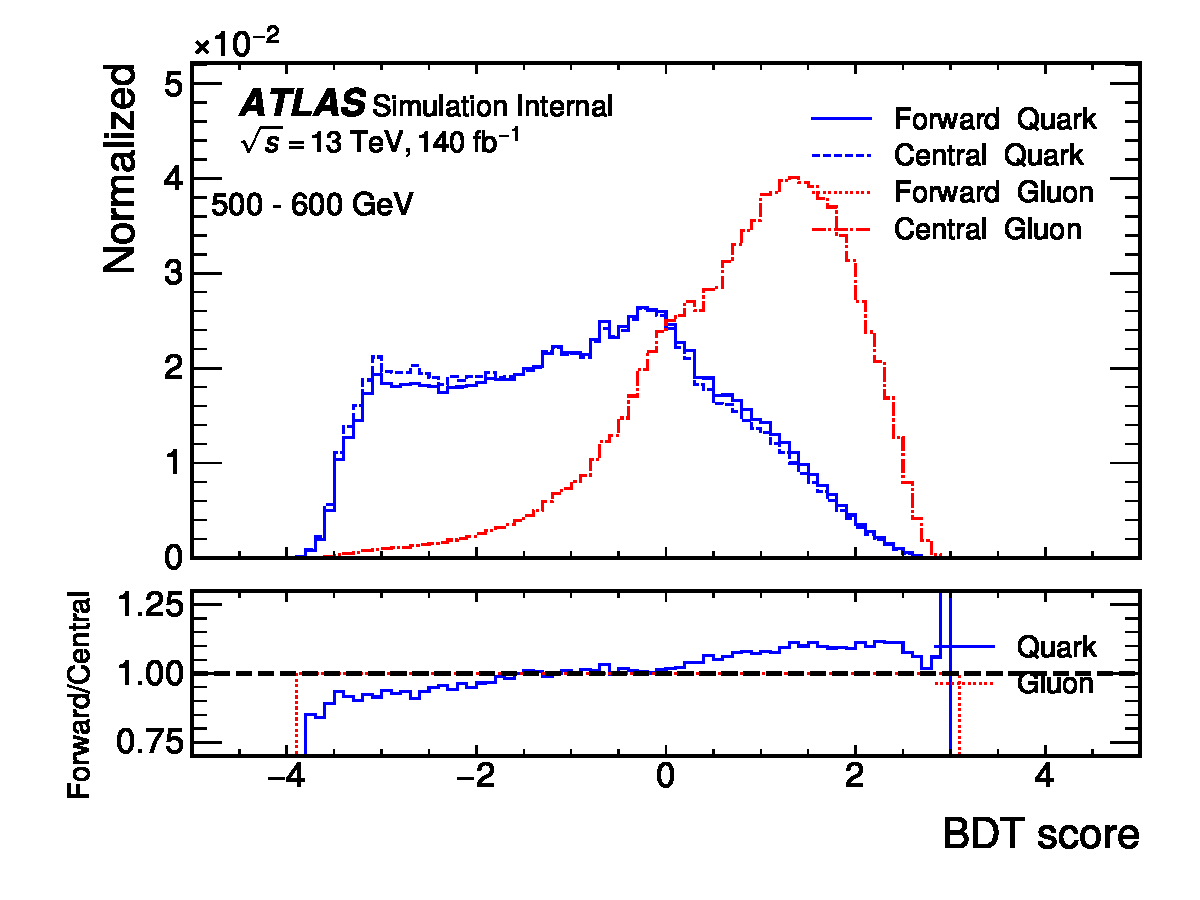
\includegraphics[width=0.45\textwidth]{fig/gluon_reweight/plots/ADE/FvsC/GBDT_newScore_quark_reweighting_weights/GBDT_newScore/MC_truth_Q_G_FvsC_500_GBDT_newScore_quark_reweighting_weights.pdf}} \quad
  	\subfloat[ ]{\label{fig:QG-pythia-GBDTMCExtractedGluonFactor-800-1000-Ntrk}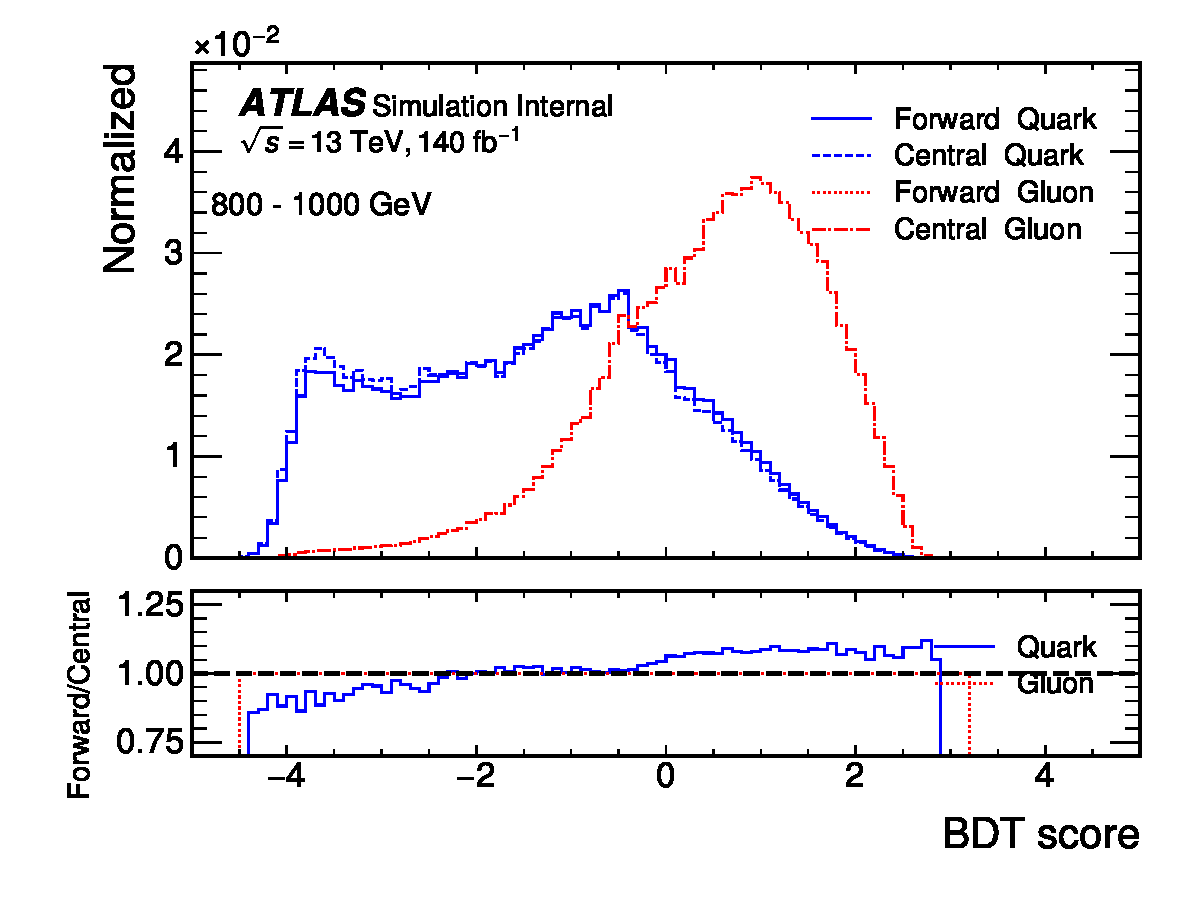
\includegraphics[width=0.45\textwidth]{fig/gluon_reweight/plots/ADE/FvsC/GBDT_newScore_quark_reweighting_weights/GBDT_newScore/MC_truth_Q_G_FvsC_800_GBDT_newScore_quark_reweighting_weights.pdf}}
  	\caption[]{
  		The distribution of BDT for jets between 500-600 GeV  \subref{fig:QG-pythia-GBDTMCExtractedGluonFactor-500-600-Ntrk} and 800-1000 GeV  \subref{fig:QG-pythia-GBDTMCExtractedGluonFactor-800-1000-Ntrk} after re-weighting using gluon factor. 
  		\label{fig:QG-pythia-GBDTMCExtracted-Reweight-Compare1_g}
  	}
  \end{figure}
  
  
  
  \begin{figure}[htb]
  	\centering
  	\subfloat[]{\label{fig:QG-pythia-NtrkDataQa}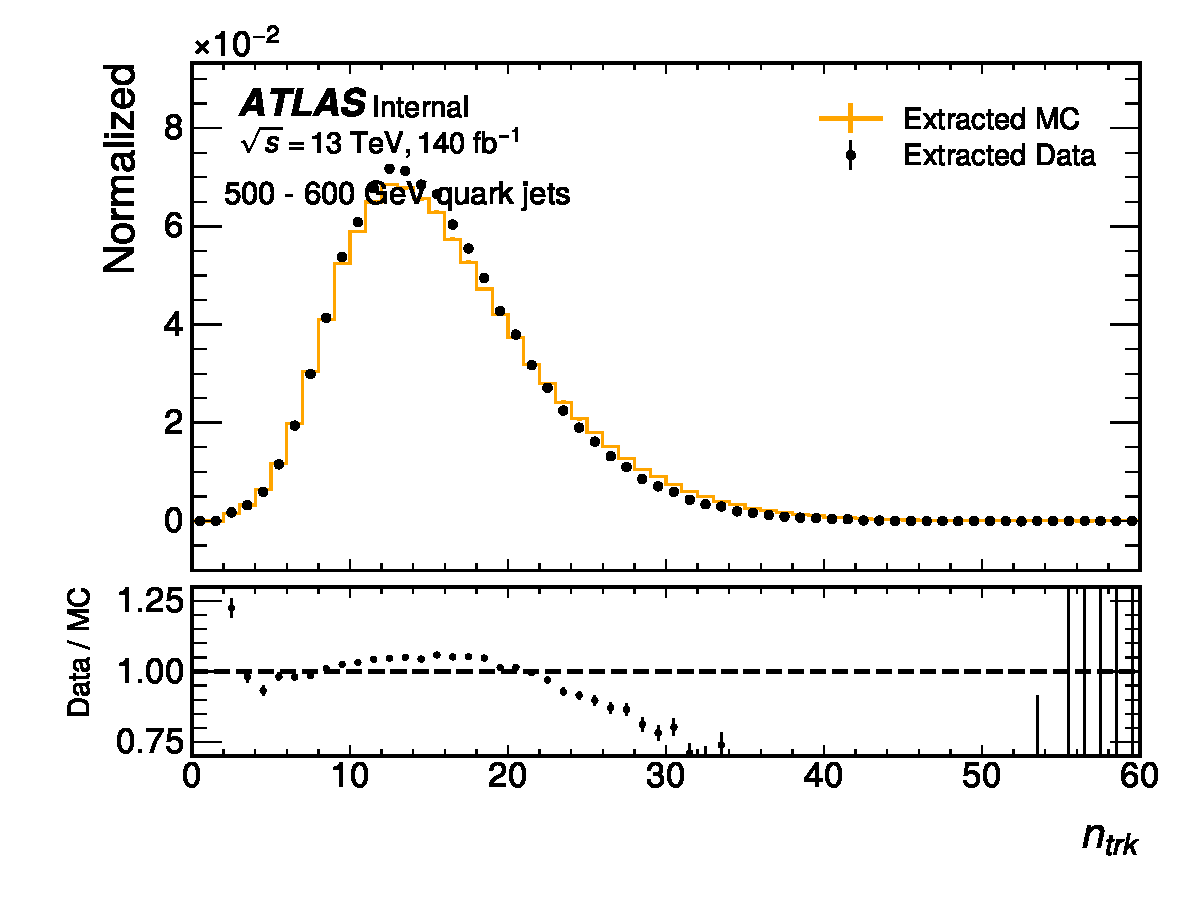
\includegraphics[width=0.45\textwidth]{fig/gluon_reweight/plots/ADE/Extractions/jet_nTracks_quark_reweighting_weights/jet_nTracks/DataExtraction_500_quark_jet_nTracks.pdf}} \quad
  	\subfloat[]{\label{fig:QG-pythia-NtrkDataG1a}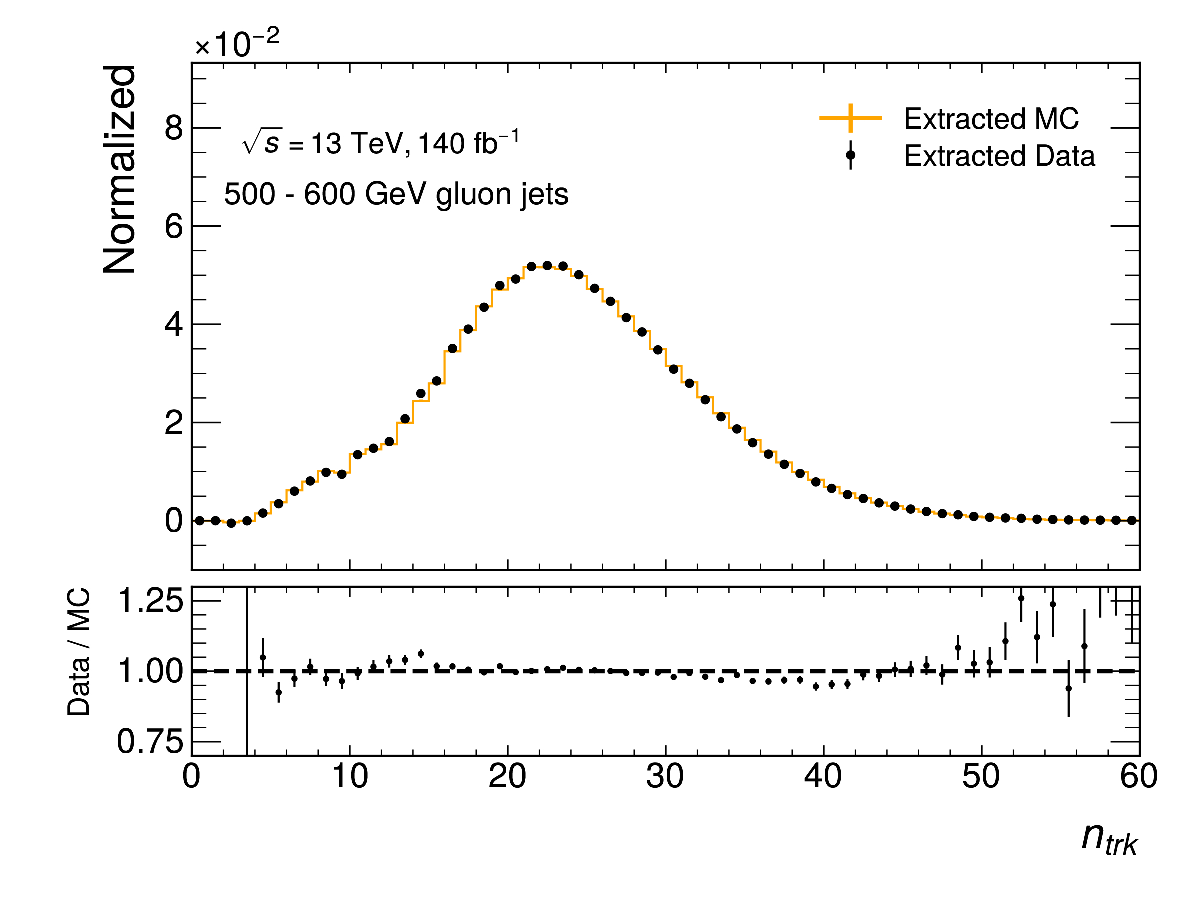
\includegraphics[width=0.45\textwidth]{fig/gluon_reweight/plots/ADE/Extractions/jet_nTracks_quark_reweighting_weights/jet_nTracks/DataExtraction_500_gluon_jet_nTracks.pdf}}  \\
  	\subfloat[]{\label{fig:QG-pythia-BDTDataQ11b}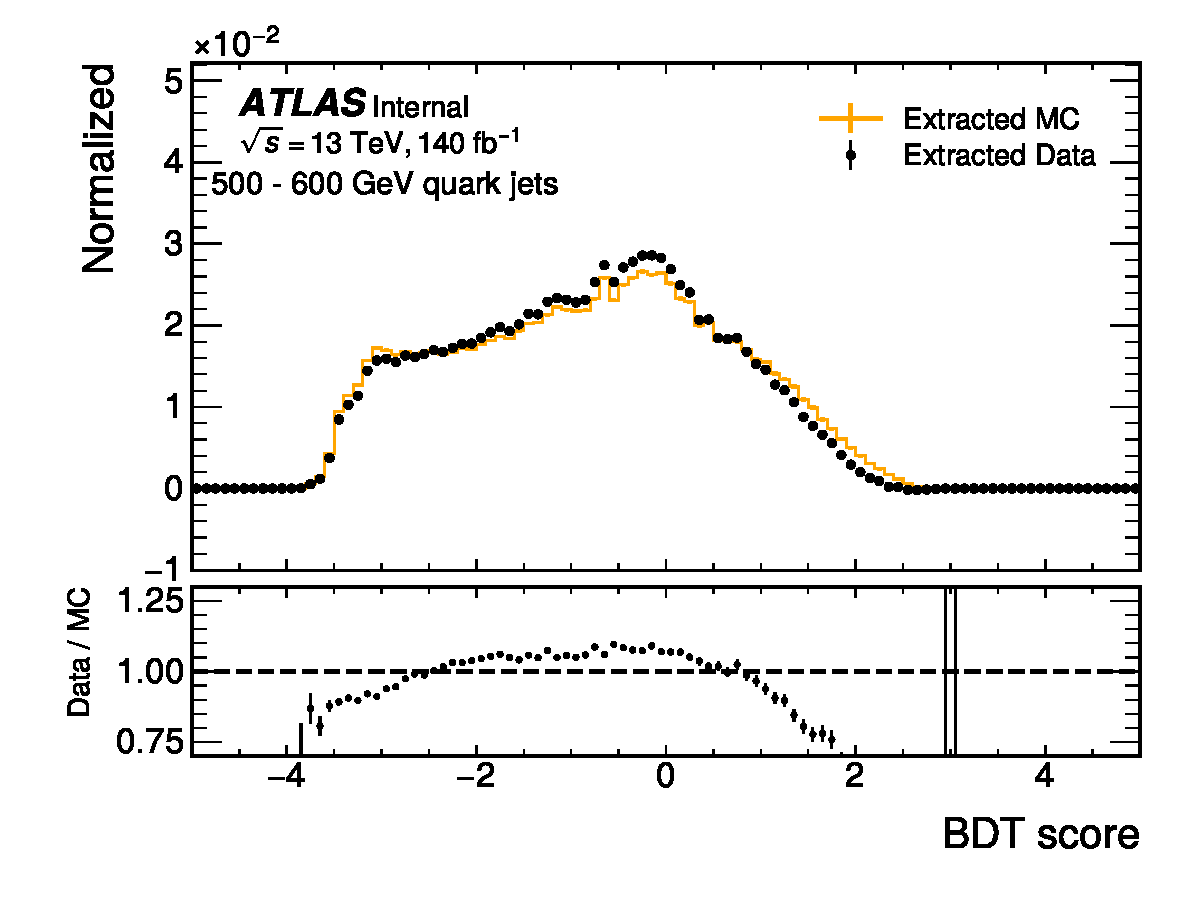
\includegraphics[width=0.45\textwidth]{fig/gluon_reweight/plots/ADE/Extractions/GBDT_newScore_quark_reweighting_weights/GBDT_newScore/DataExtraction_500_quark_GBDT_newScore.pdf}} \quad
  	\subfloat[]{\label{fig:QG-pythia-BDTDataG1b}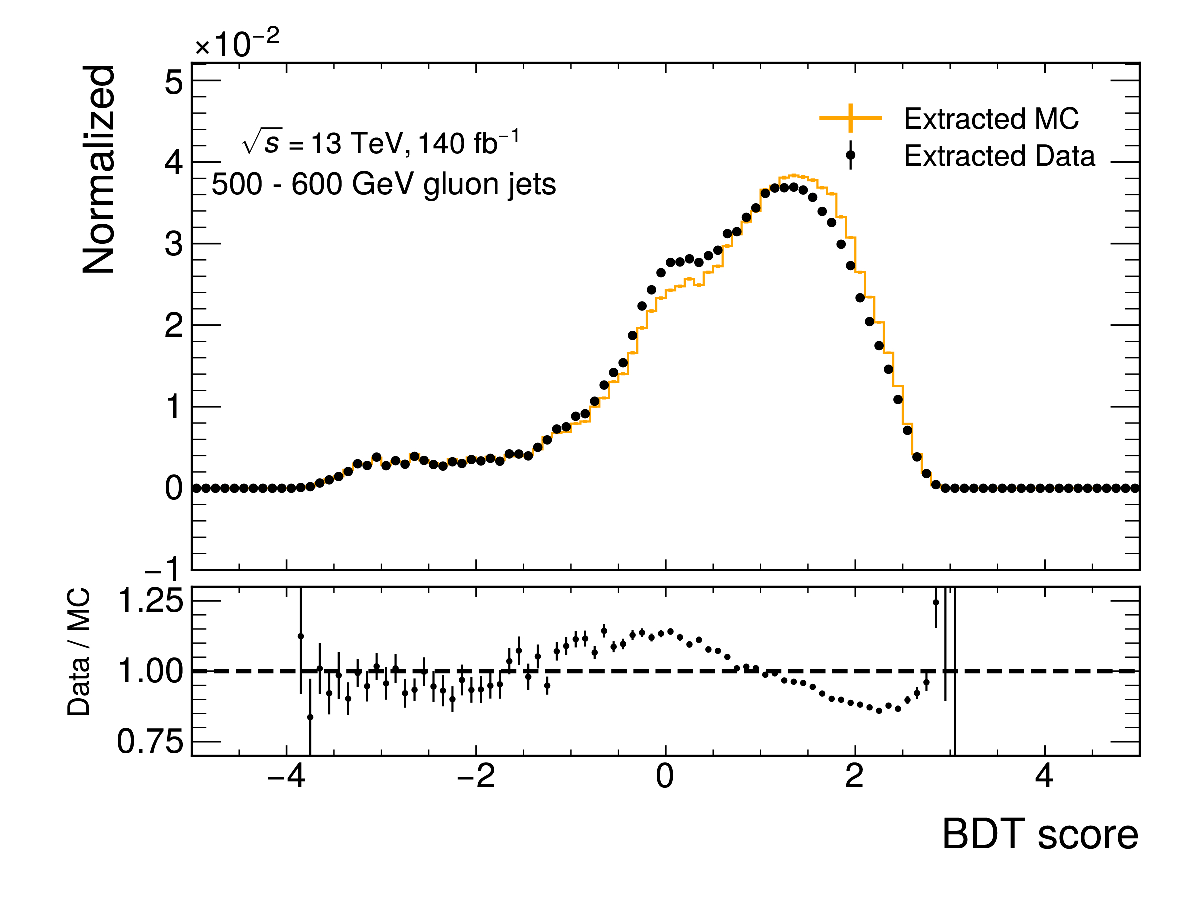
\includegraphics[width=0.45\textwidth]{fig/gluon_reweight/plots/ADE/Extractions/GBDT_newScore_quark_reweighting_weights/GBDT_newScore/DataExtraction_500_gluon_GBDT_newScore.pdf}} \\
  	\caption[]{
  		The \ntrk~(top) and BDT (bottom) distributions extracted by the matrix method from the data and MC of pure quark-jets \subref{fig:QG-pythia-NtrkDataQa} \subref{fig:QG-pythia-BDTDataQ11b} and  gluon-jets \subref{fig:QG-pythia-NtrkDataGa} \subref{fig:QG-pythia-BDTDataG1b} by \pythia8. %
  		extracted by the matrix method from the data and MC. The gluon factor is applied. %
  		Solid-line histograms show the distributions of quark or gluon-jets defined by the jet parton flavour label in the MC.
  		A bottom panel in each figure shows the ratio of the extracted data to the extracted MC by the matrix method. %
  		\label{fig:QG-pythia-NtrkData500Gluon}
  	}
  \end{figure}
  
  
  \begin{figure}[htb]
  	\centering
  	\subfloat[]{\label{fig:QG-pythia-NtrkDataQa11}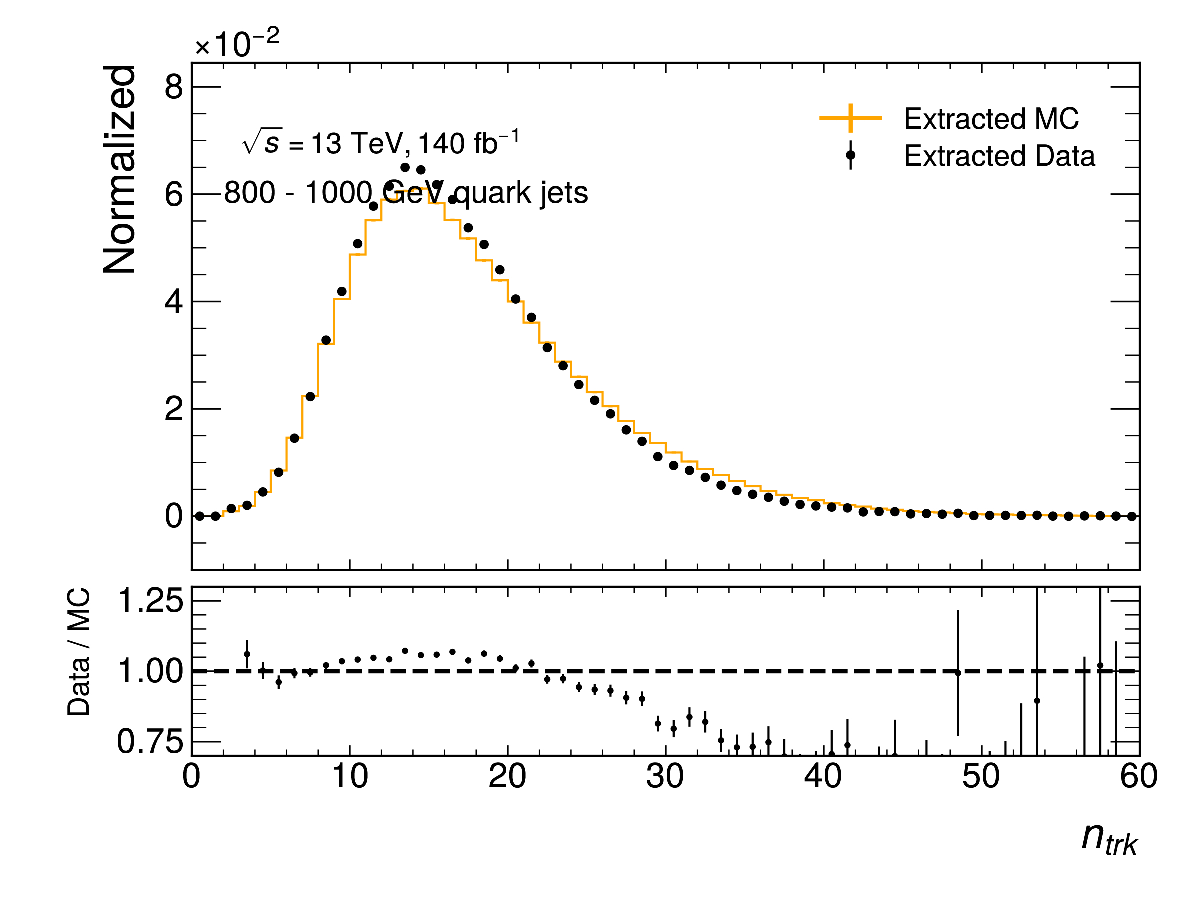
\includegraphics[width=0.45\textwidth]{fig/gluon_reweight/plots/ADE/Extractions/jet_nTracks_quark_reweighting_weights/jet_nTracks/DataExtraction_800_quark_jet_nTracks.pdf}} \quad
  	\subfloat[]{\label{fig:QG-pythia-NtrkDataGa111}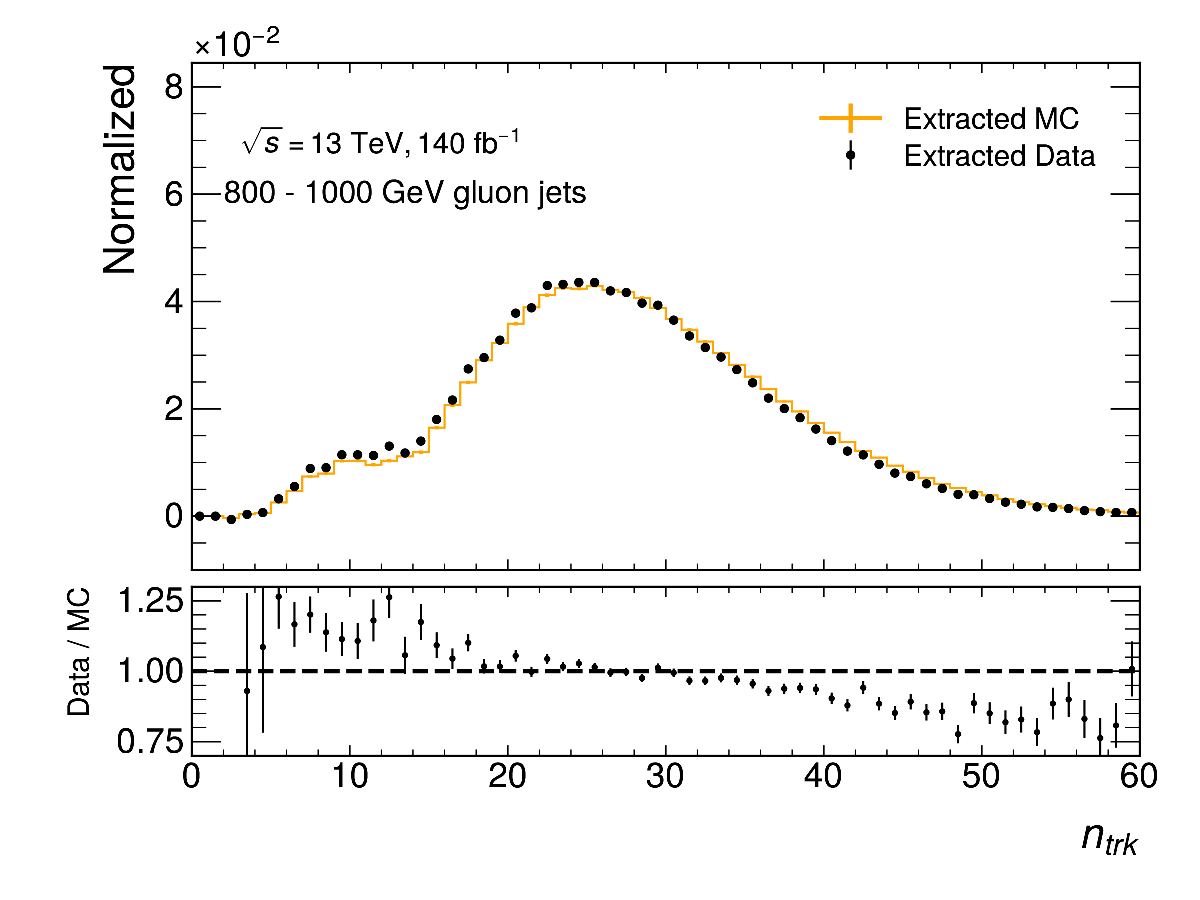
\includegraphics[width=0.45\textwidth]{fig/gluon_reweight/plots/ADE/Extractions/jet_nTracks_quark_reweighting_weights/jet_nTracks/DataExtraction_800_gluon_jet_nTracks.pdf}}  \\
  	\subfloat[]{\label{fig:QG-pythia-BDTDataQb11}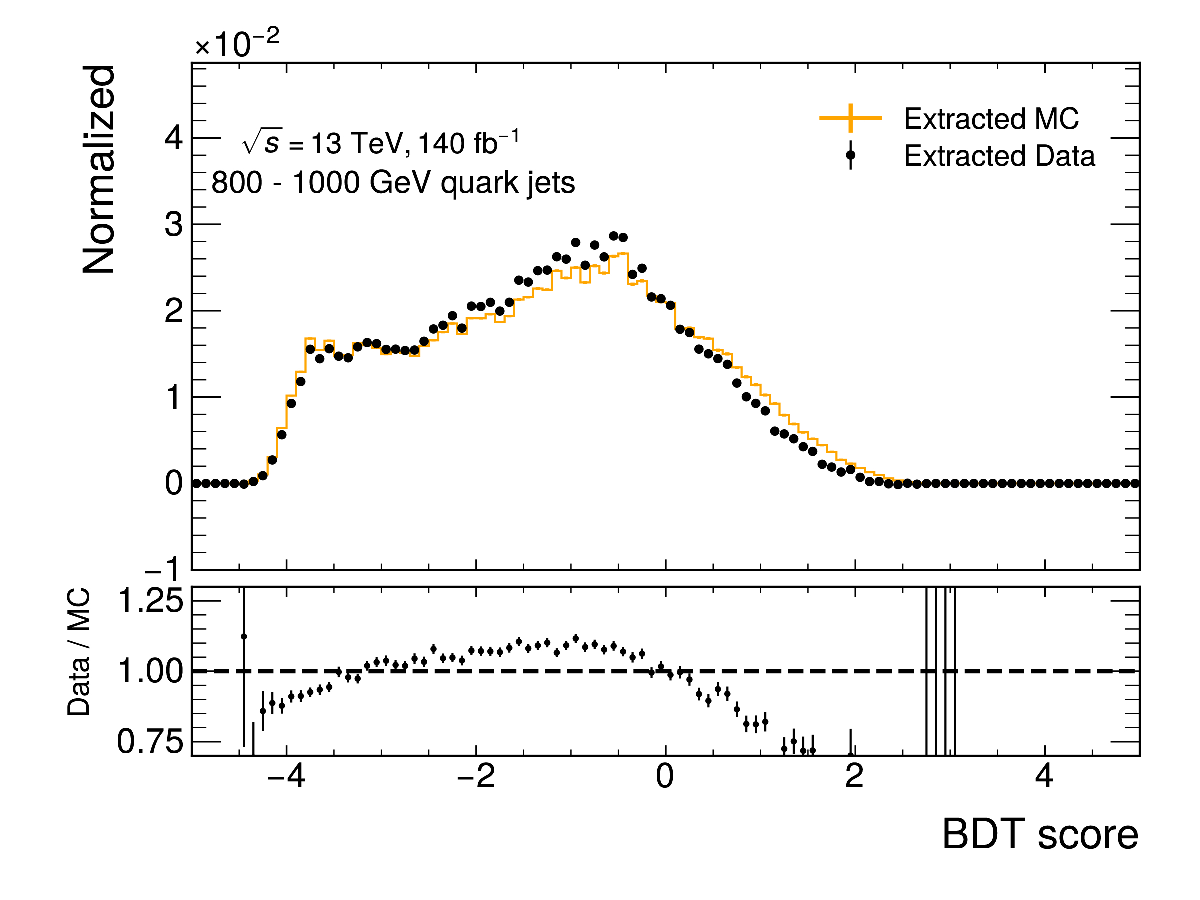
\includegraphics[width=0.45\textwidth]{fig/gluon_reweight/plots/ADE/Extractions/GBDT_newScore_quark_reweighting_weights/GBDT_newScore/DataExtraction_800_quark_GBDT_newScore.pdf}} \quad
  	\subfloat[]{\label{fig:QG-pythia-BDTDataGb111}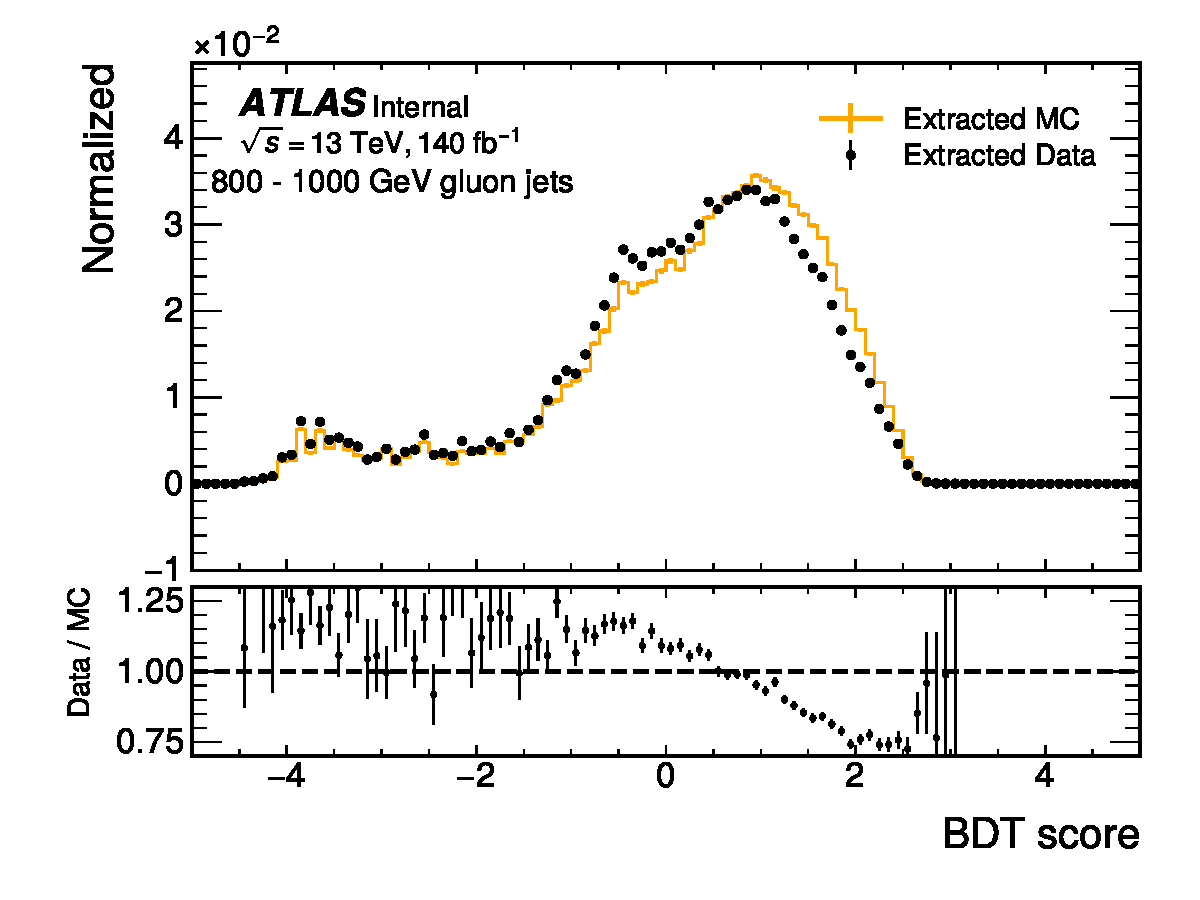
\includegraphics[width=0.45\textwidth]{fig/gluon_reweight/plots/ADE/Extractions/GBDT_newScore_quark_reweighting_weights/GBDT_newScore/DataExtraction_800_gluon_GBDT_newScore.pdf}} \\
  	\caption[]{
  		The \ntrk~(top) and BDT (bottom) distributions extracted by the matrix method from the data and MC of pure quark-jets \subref{fig:QG-pythia-NtrkDataQa11} \subref{fig:QG-pythia-BDTDataQb11} and  gluon-jets \subref{fig:QG-pythia-NtrkDataGa111} \subref{fig:QG-pythia-BDTDataGb111}  by \pythia8. %
  		extracted by the matrix method from the data and MC.The gluon factor is applied. Solid-line histograms show the distributions of quark or gluon-jets defined by the jet parton flavour label in the MC.
  		A bottom panel in each figure shows the ratio of the extracted data to the extracted MC by the matrix method. %
  		\label{fig:QG-pythia-NtrkData800Gluon}
  	}
  \end{figure}
  
  \FloatBarrier
  
    \subsubsection{The MC non-closure}
   As described in Section.~\ref{sec:QG-closure}, the MC closure test is conducted using MC samples wherein each jet is assigned a truth label. After re-weighting, the distributions of {\ntrk} and BDT obtained through the matrix method exhibit consistency with the truth-labelled ones for quark- and gluon-jets, respectively. The remaining difference for both taggers is only 1\% level.



    \subsubsection{Statistical uncertainty}
 The estimation of statistical uncertainty involves a stepwise process. It commences by varying the input data/MC distributions bin-by-bin, using Poisson/Gaussian distributions wherein the number of data events within each bin serves as the central value. These variations of the input histograms yield templates, subsequently employed as inputs for the template variations technique. This procedure is iterated 5000 times, with the standard deviation of these uncertainties of all toys taken is used to derive the statistical uncertainty of the SFs. This uncertainty is around 0.1\%.
    
   The distributions of SFs are shown in \ref{fig:QG-pythia-bootstrap-500-ntrk} for \ntrk~and \ref{fig:QG-pythia-bootstrap-500-bdt} for the BDT.  
  \begin{figure}[htb]
	\centering
	\subfloat[working Point:50\%~(Quark)]{\label{fig:QG-pythia-BDTQ5}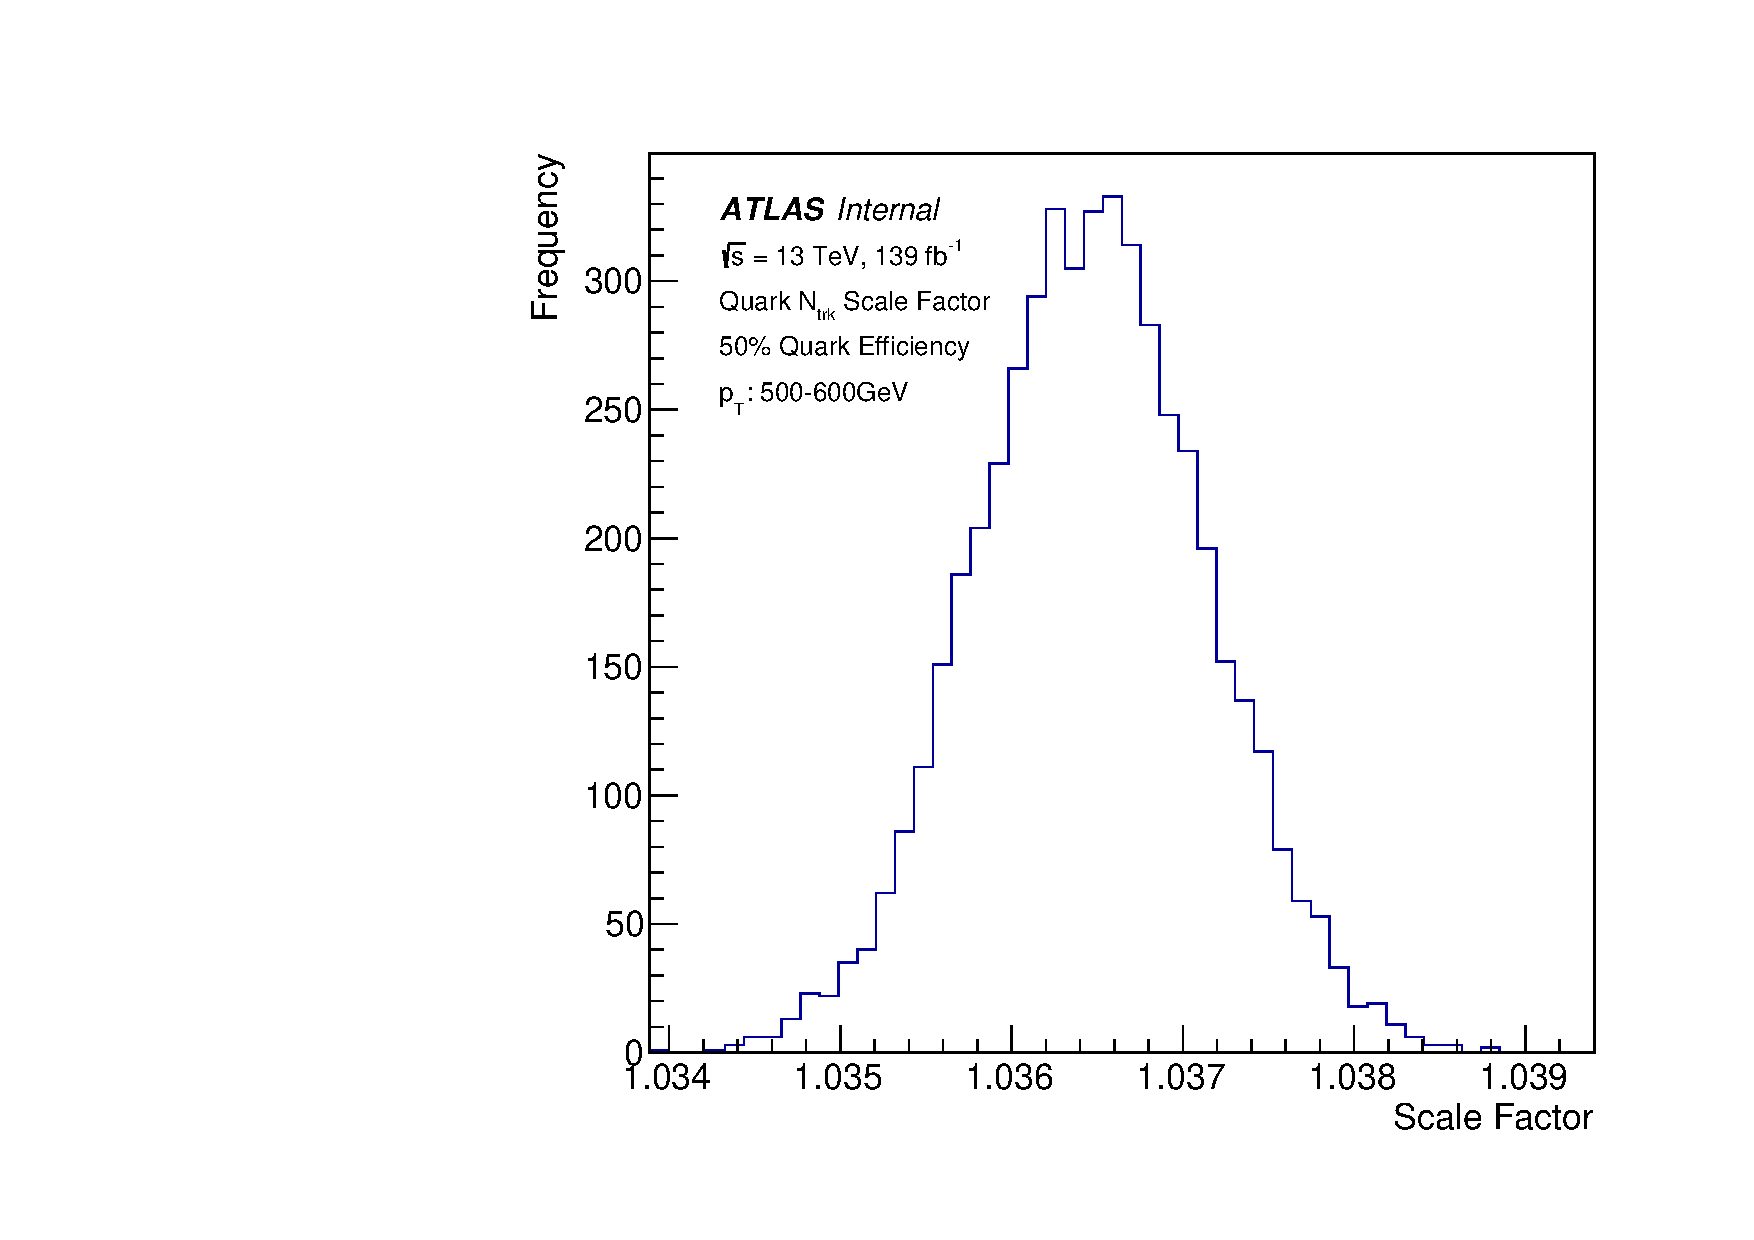
\includegraphics[width=0.22\textwidth]{fig/Method1/pythia/Bootstrap/500-0.5-ntrk-quark.pdf}} \quad
	\subfloat[working Point:60\%~(Quark)]{\label{fig:QG-pythia-BDTQ6}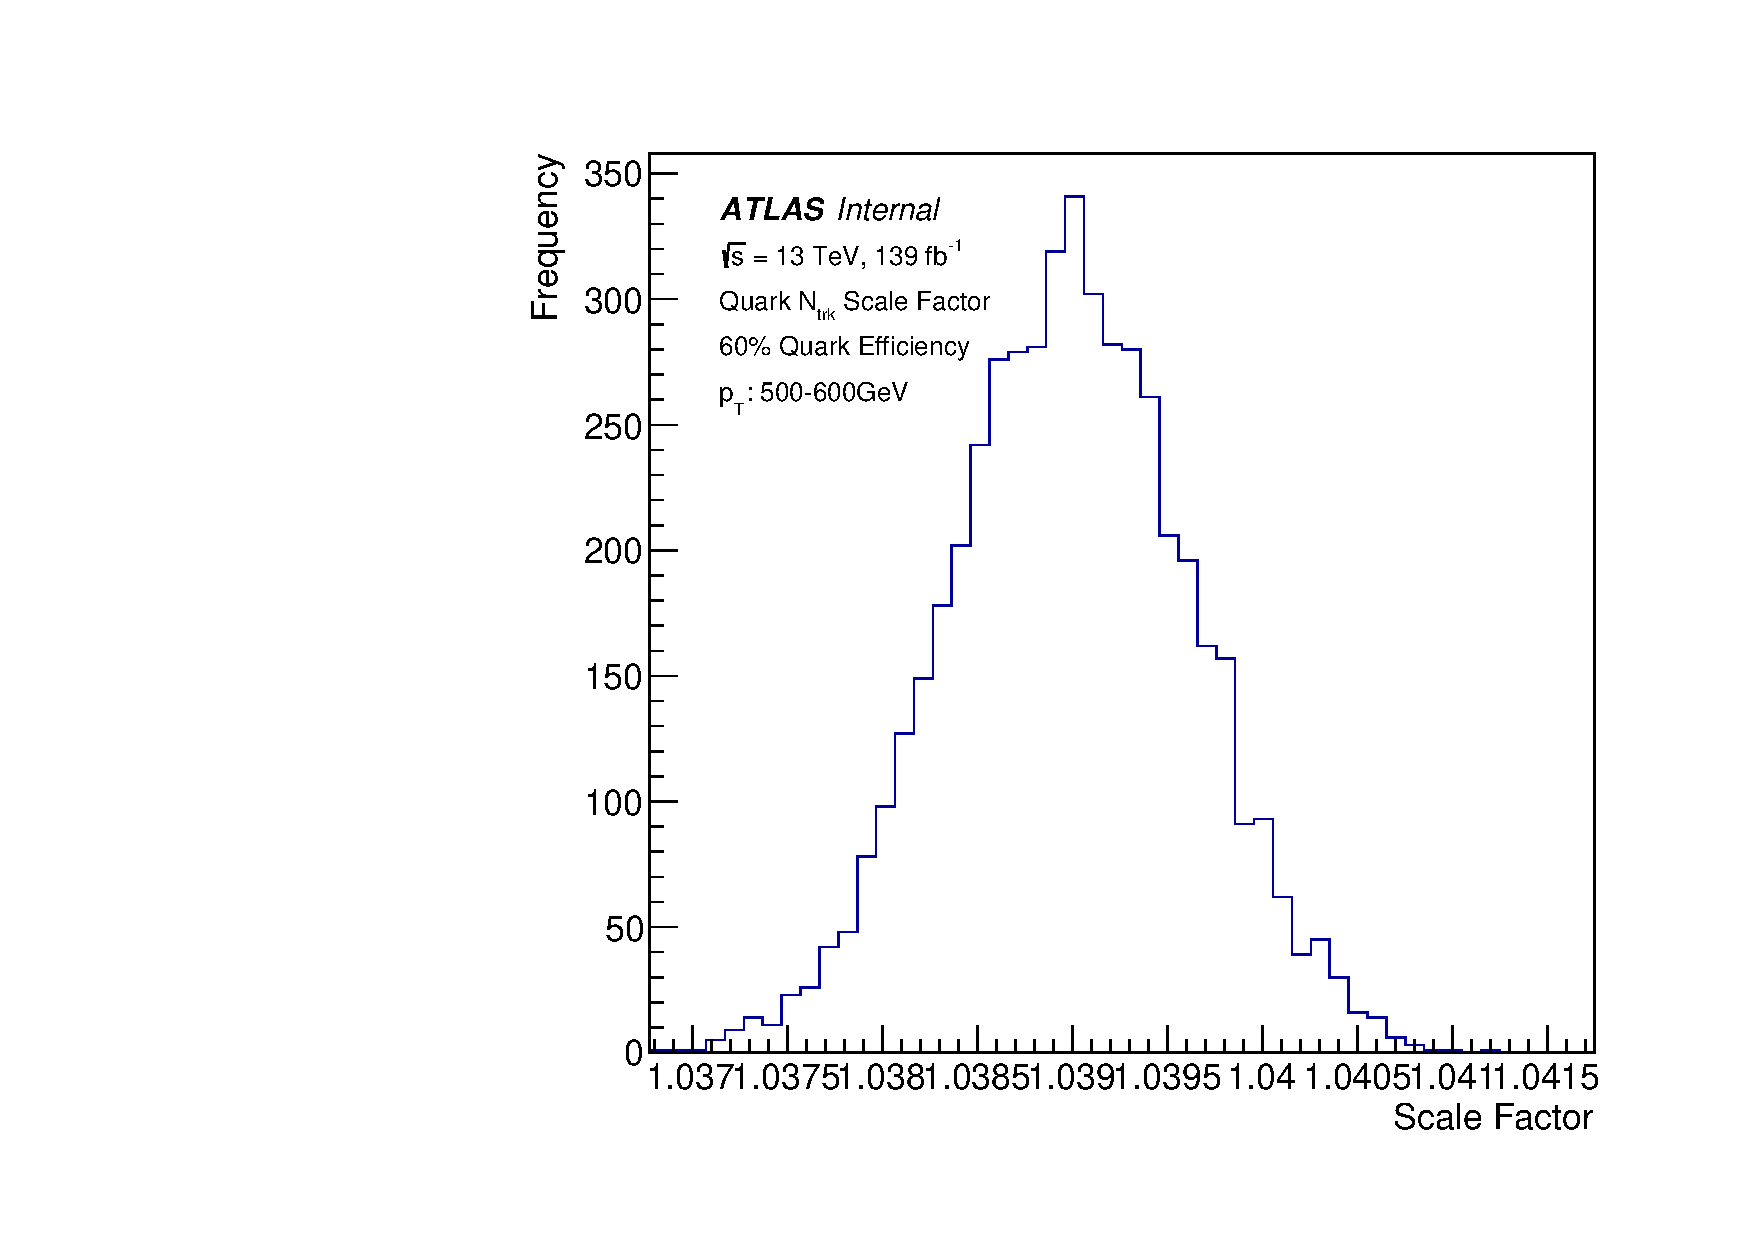
\includegraphics[width=0.22\textwidth]{fig/Method1/pythia/Bootstrap/500-0.6-ntrk-quark.pdf}}\quad
	\subfloat[working Point:70\%~(Quark)]{\label{fig:QG-pythia-BDTQ7}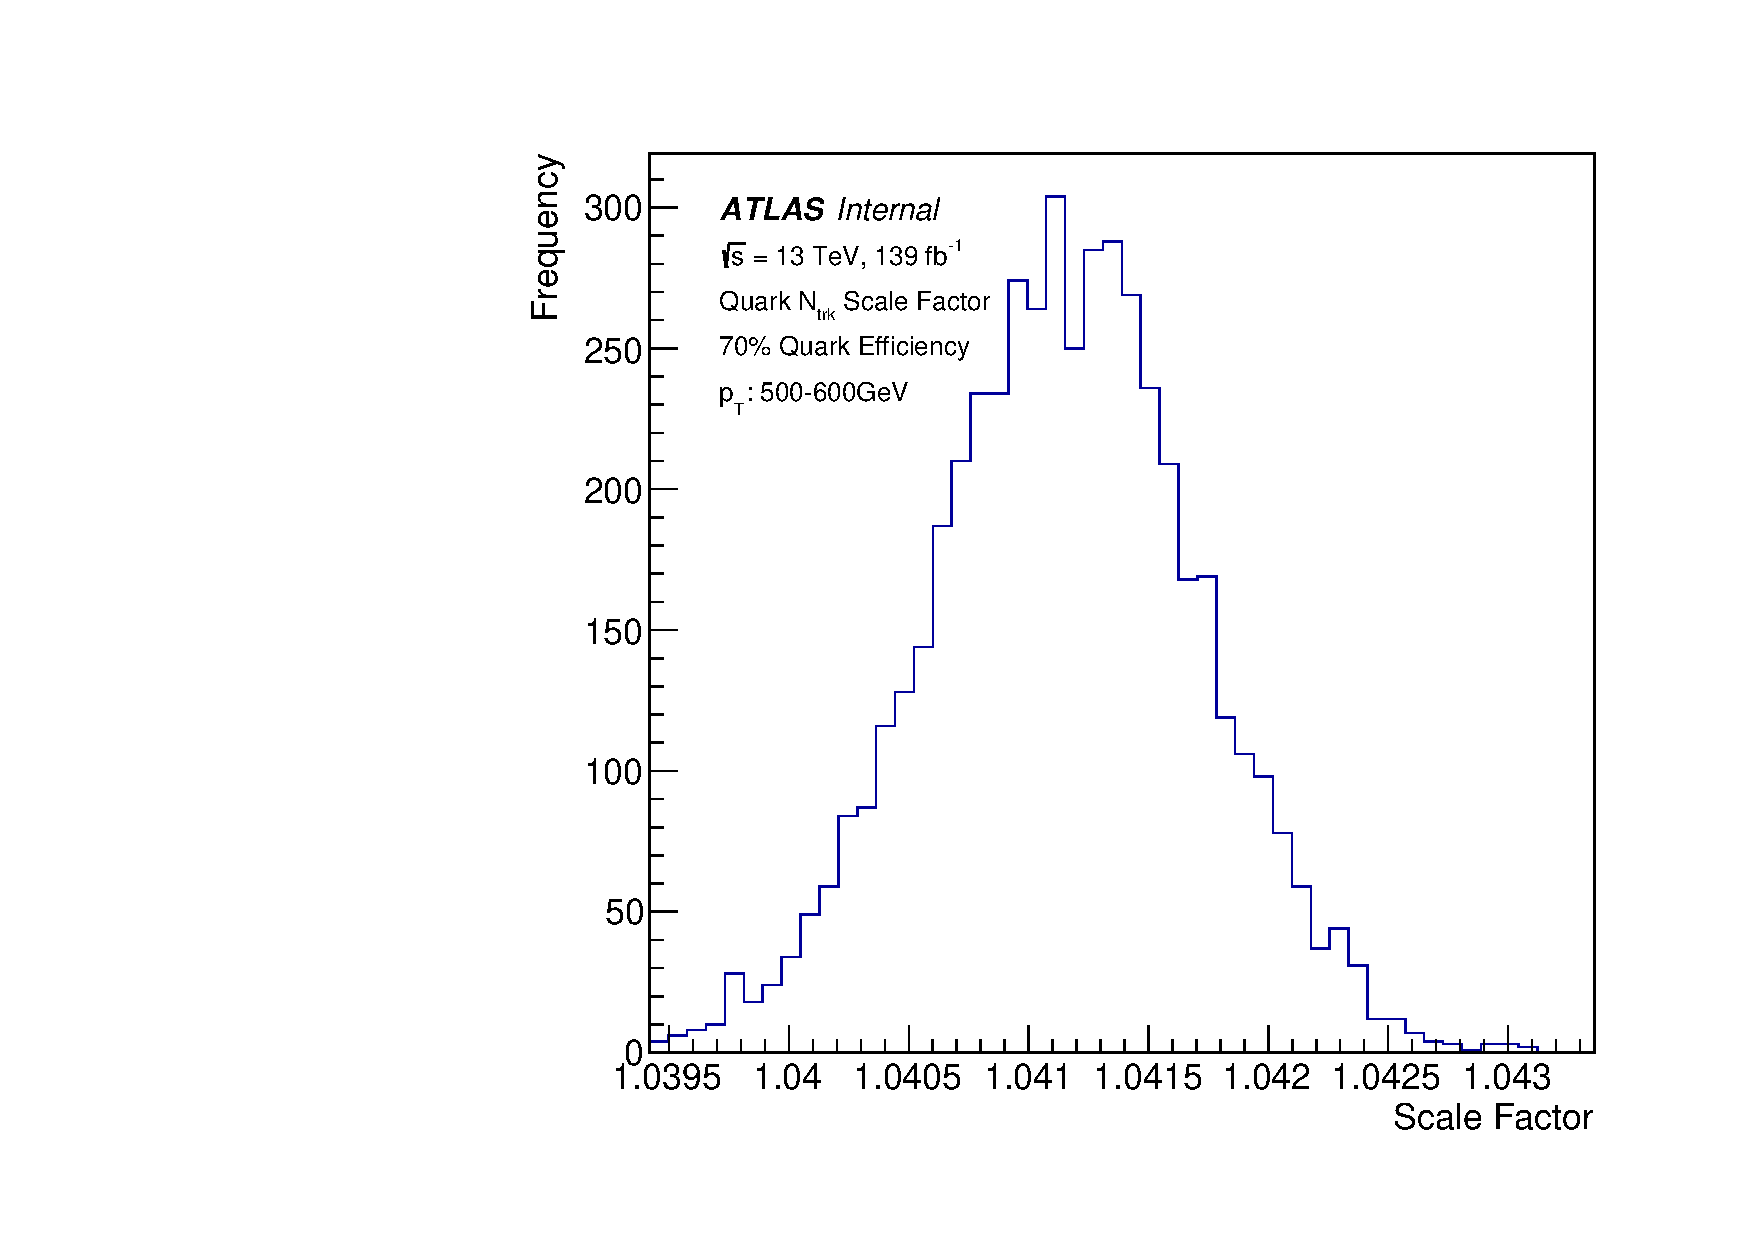
\includegraphics[width=0.22\textwidth]{fig/Method1/pythia/Bootstrap/500-0.7-ntrk-quark.pdf}} \quad
	\subfloat[working Point:80\%~(Quark)]{\label{fig:QG-pythia-BDTQ8}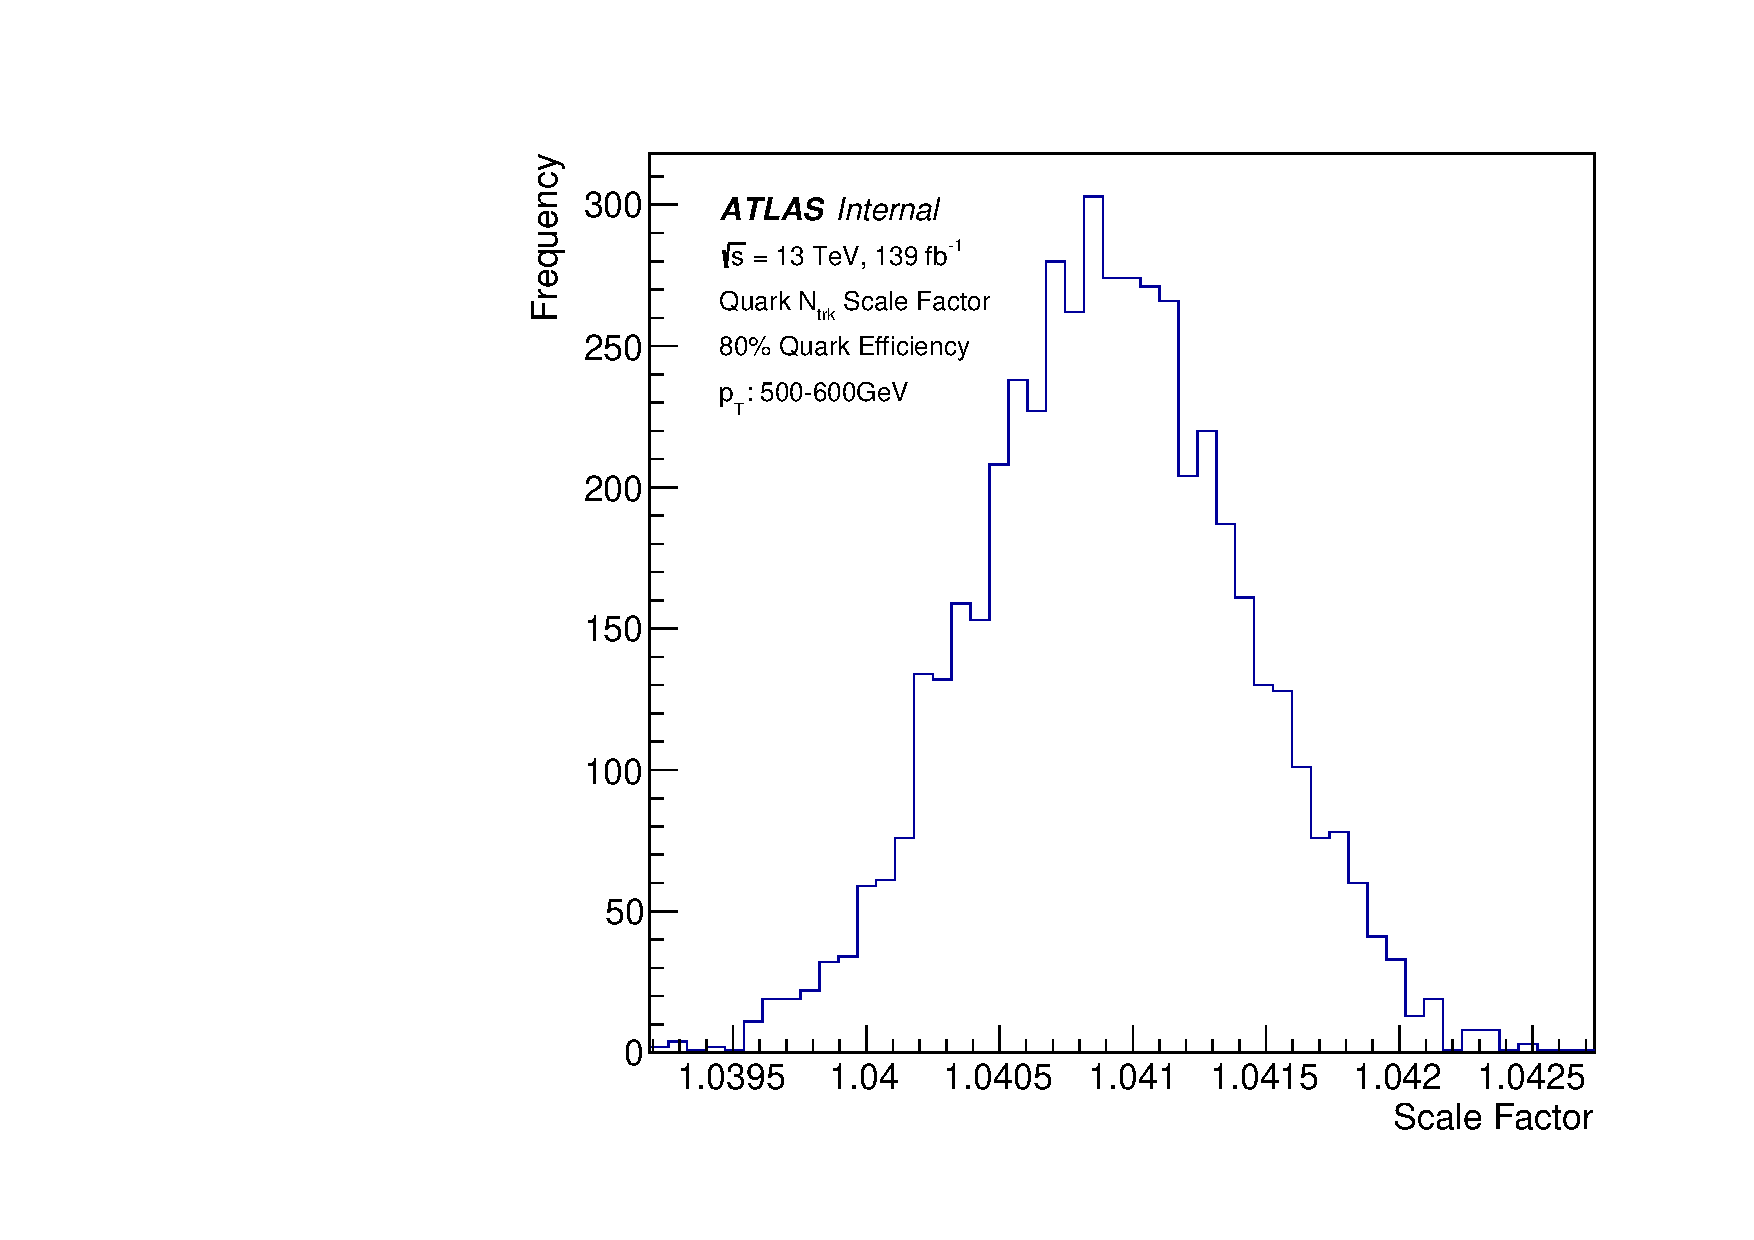
\includegraphics[width=0.22\textwidth]{fig/Method1/pythia/Bootstrap/500-0.8-ntrk-quark.pdf}}\\
	\subfloat[working Point:50\%~(Gluon)]{\label{fig:QG-pythia-BDTG5}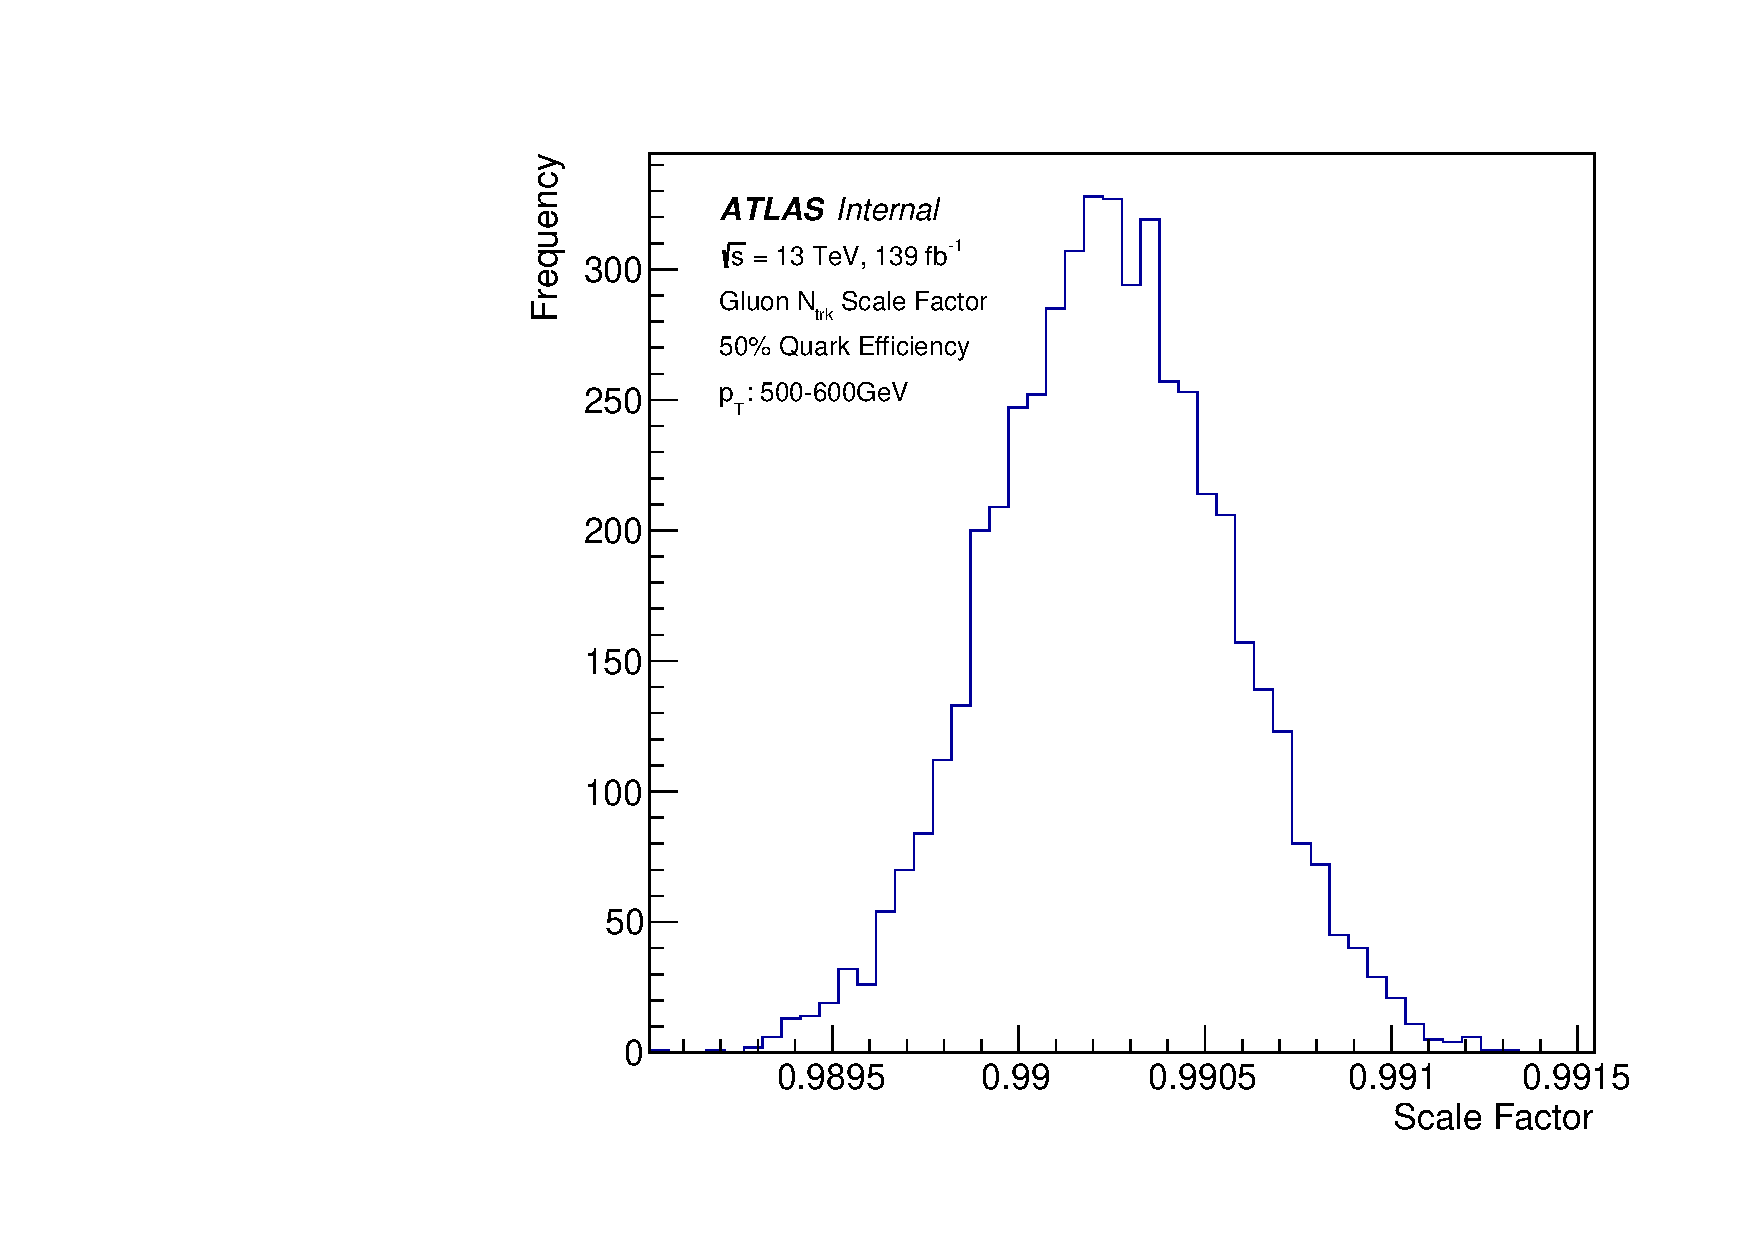
\includegraphics[width=0.22\textwidth]{fig/Method1/pythia/Bootstrap/500-0.5-ntrk-gluon.pdf}} \quad
	\subfloat[working Point:60\%~(Gluon)]{\label{fig:QG-pythia-BDTG6}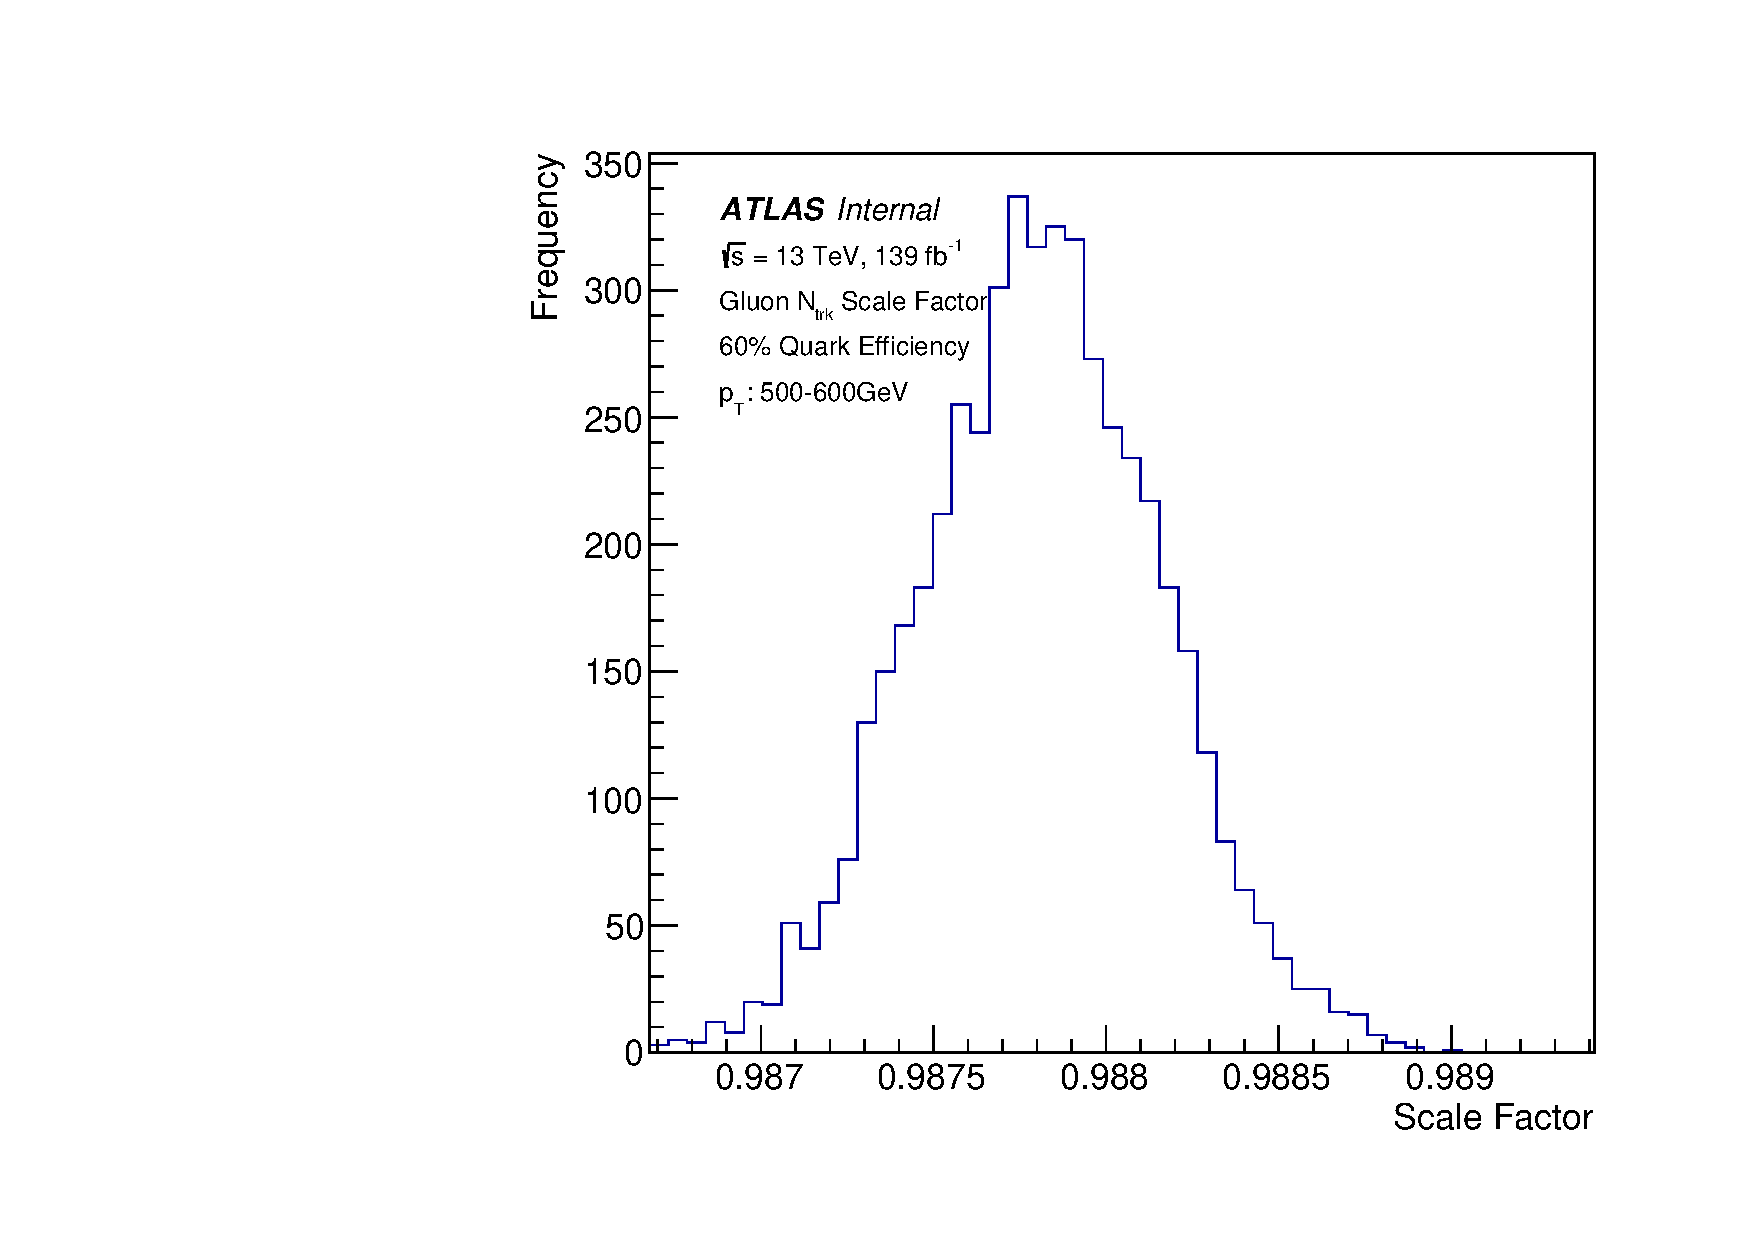
\includegraphics[width=0.22\textwidth]{fig/Method1/pythia/Bootstrap/500-0.6-ntrk-gluon.pdf}}\quad
	\subfloat[working Point:70\%~(Gluon)]{\label{fig:QG-pythia-BDTG7}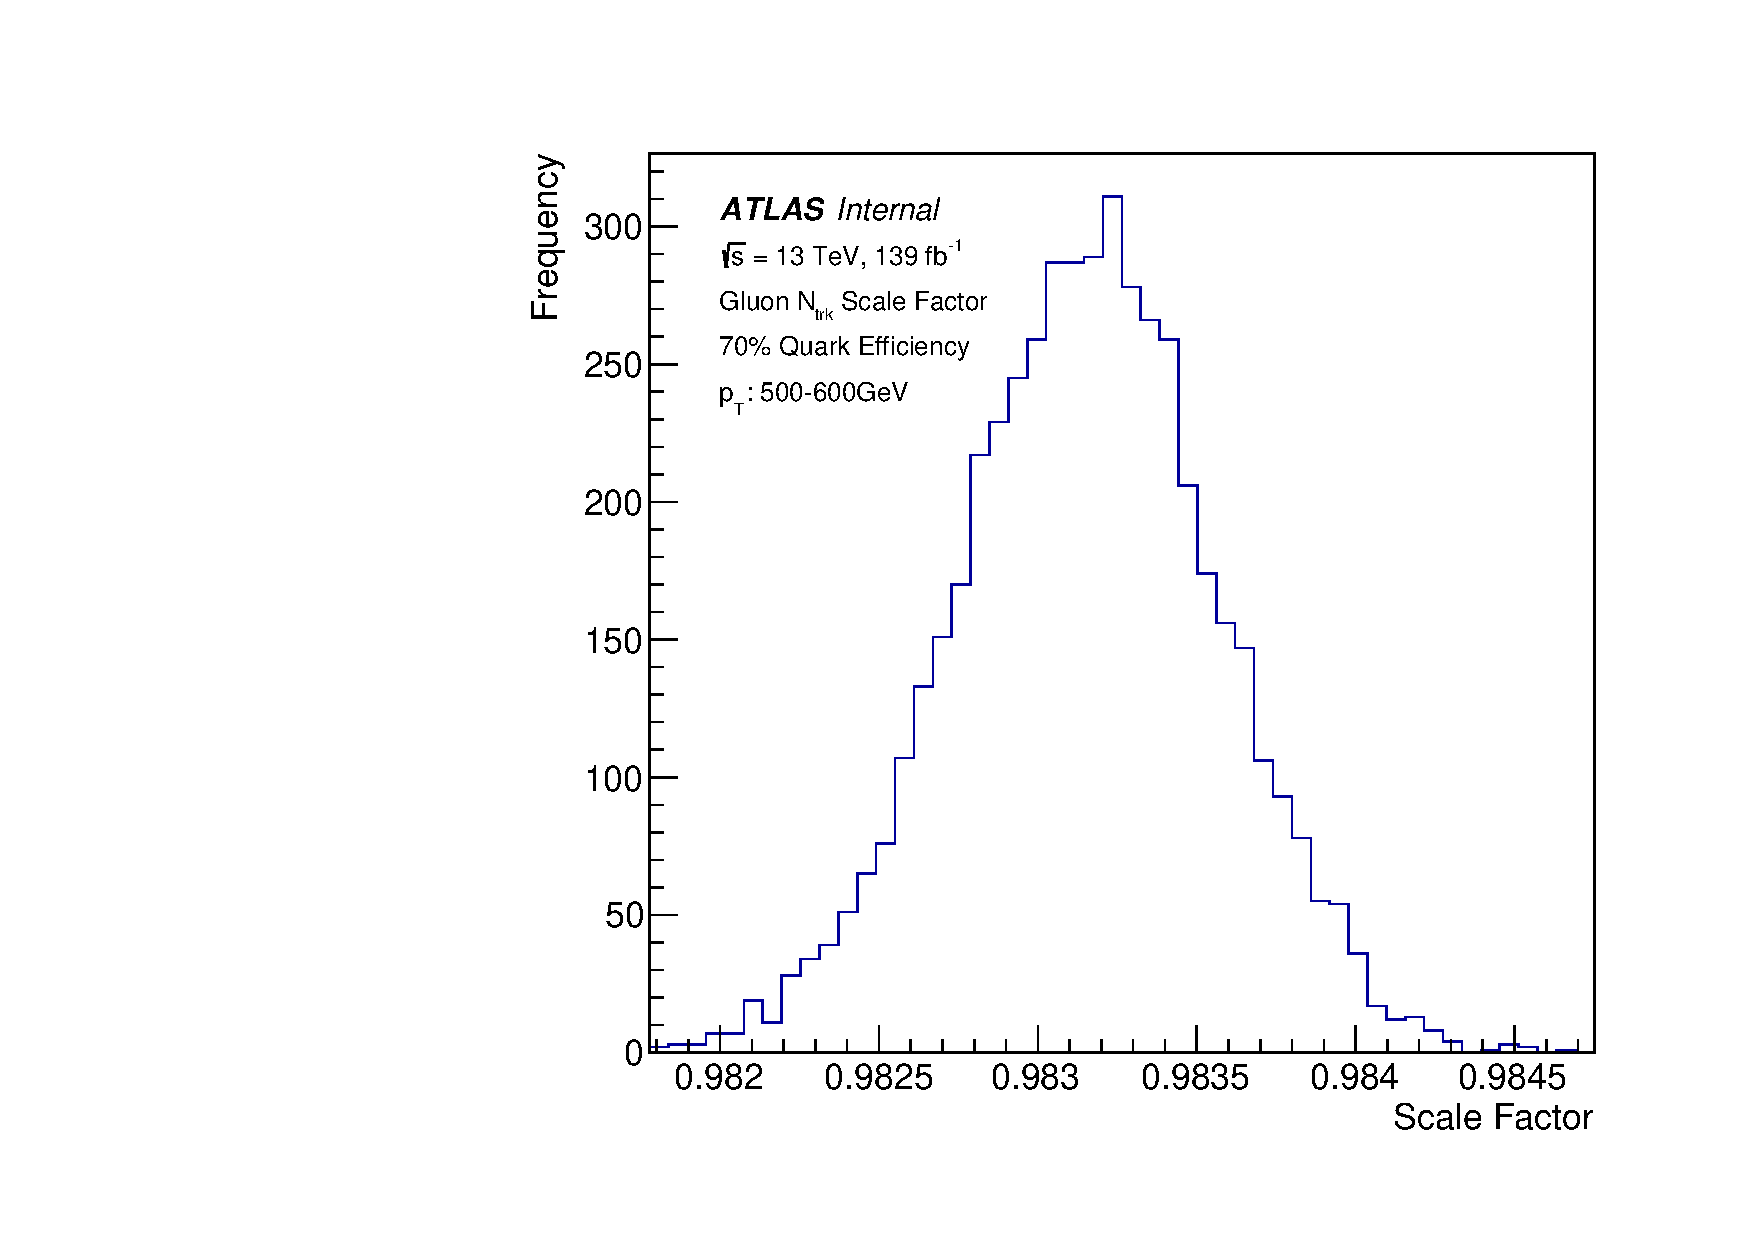
\includegraphics[width=0.22\textwidth]{fig/Method1/pythia/Bootstrap/500-0.7-ntrk-gluon.pdf}} \quad
	\subfloat[working Point:80\%~(Gluon)]{\label{fig:QG-pythia-BDTG8}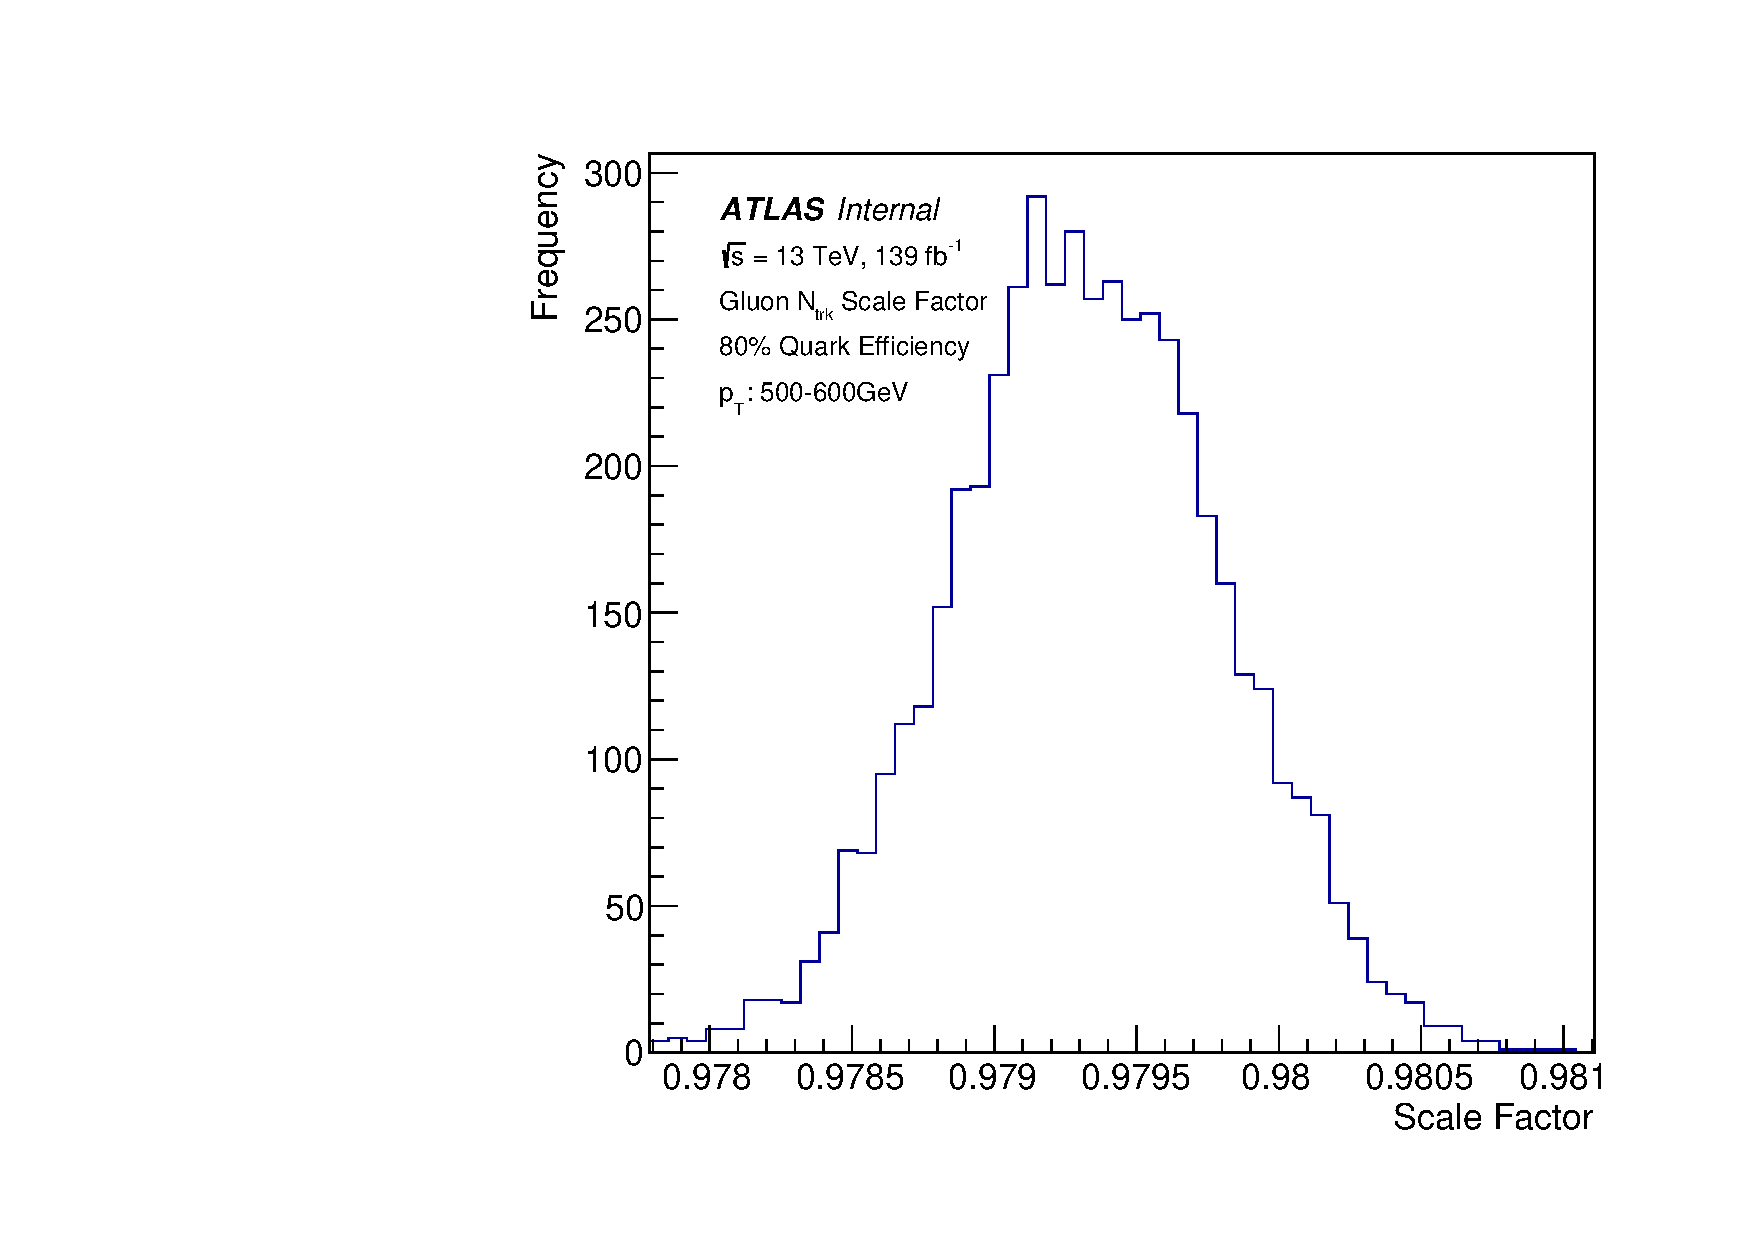
\includegraphics[width=0.22\textwidth]{fig/Method1/pythia/Bootstrap/500-0.8-ntrk-gluon.pdf}}\\
	\caption[]{
	The distribution of SF by varying the input data distributions bin-by-bin using a Poisson distribution with the number of data events in each bin as the central value for 5000 times for working point of \ntrk~in jet \pt~range 500-600 GeV. 

		\label{fig:QG-pythia-bootstrap-500-ntrk}
	}
\end{figure}



\begin{figure}[htb]
	\centering
	\subfloat[working Point:50\%~(Quark)]{\label{fig:QG-pythia-BDTQ5}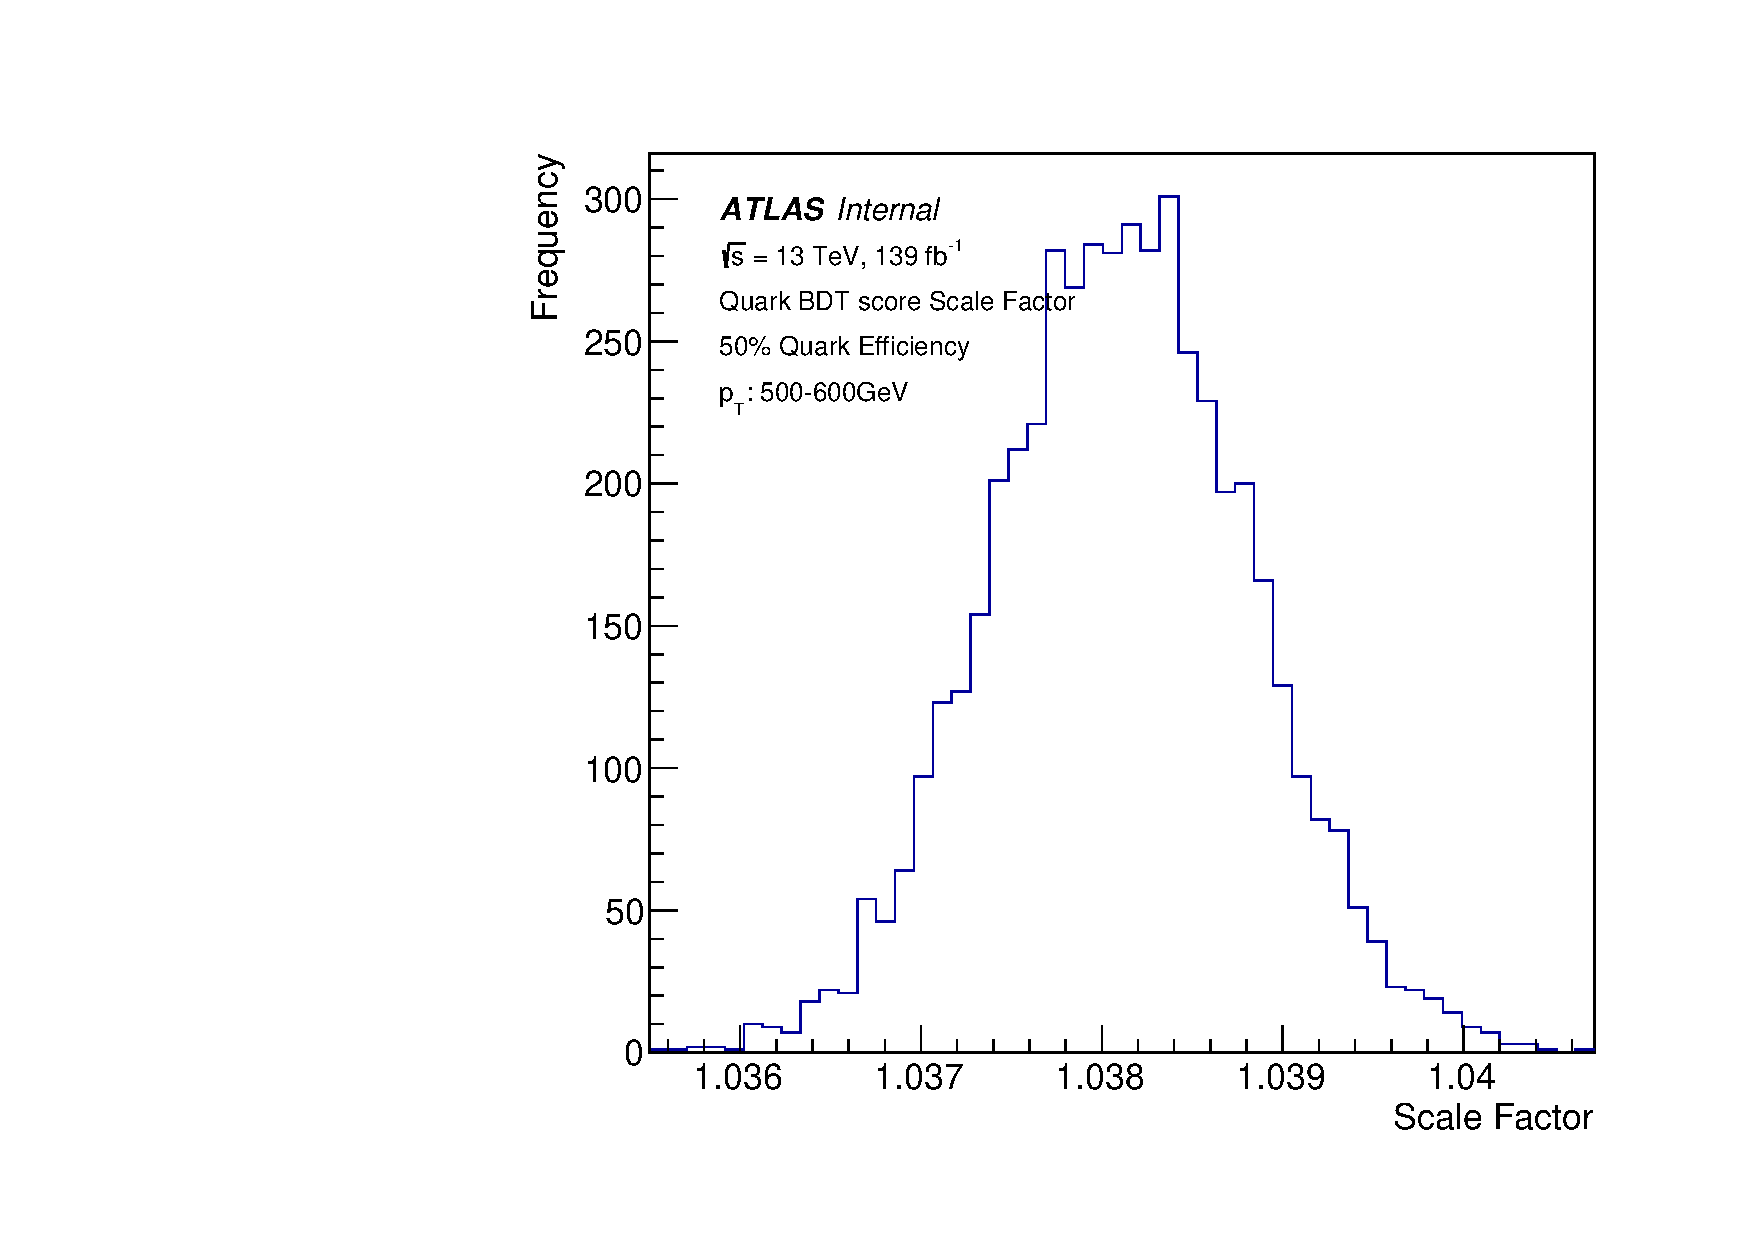
\includegraphics[width=0.22\textwidth]{fig/Method1/pythia/Bootstrap/500-0.5-bdt-quark.pdf}} \quad
	\subfloat[working Point:60\%~(Quark)]{\label{fig:QG-pythia-BDTQ6}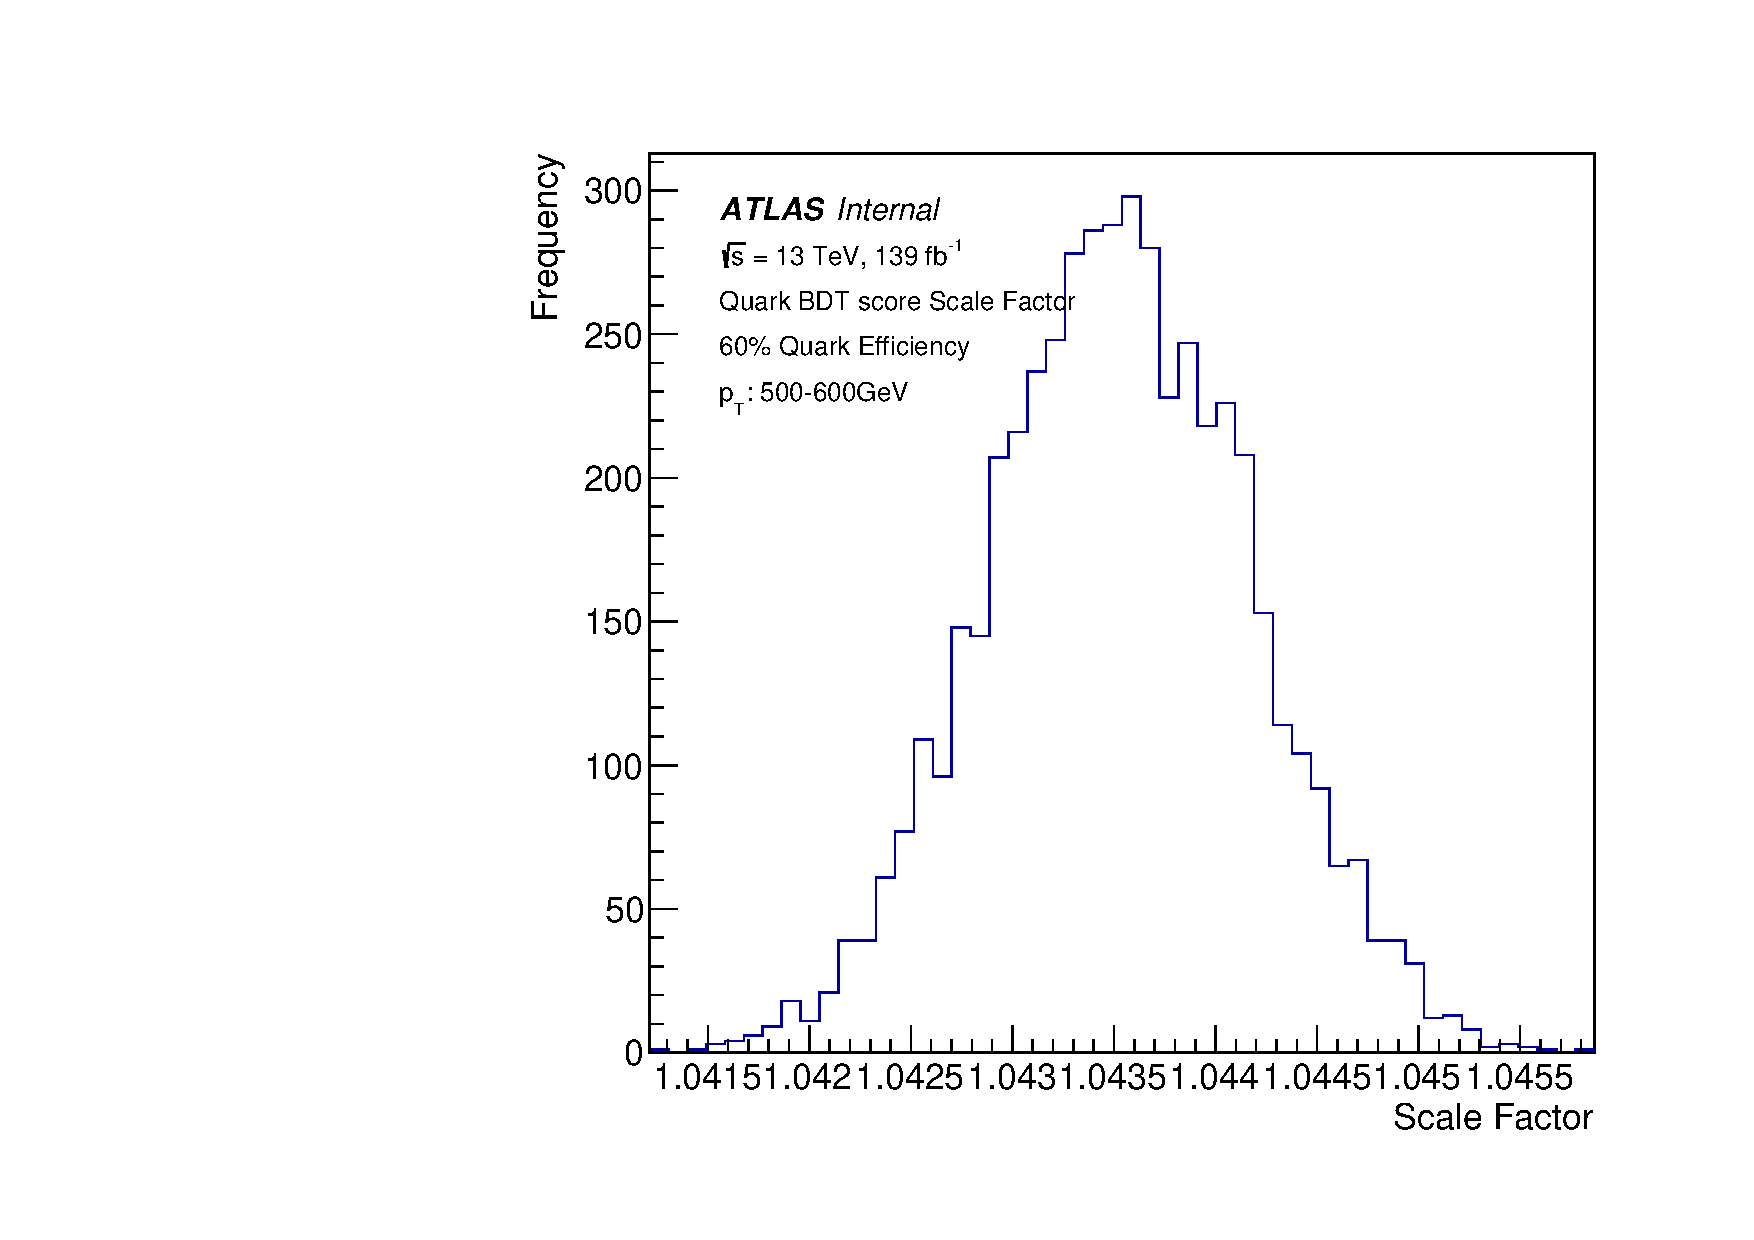
\includegraphics[width=0.22\textwidth]{fig/Method1/pythia/Bootstrap/500-0.6-bdt-quark.pdf}}\quad
	\subfloat[working Point:70\%~(Quark)]{\label{fig:QG-pythia-BDTQ7}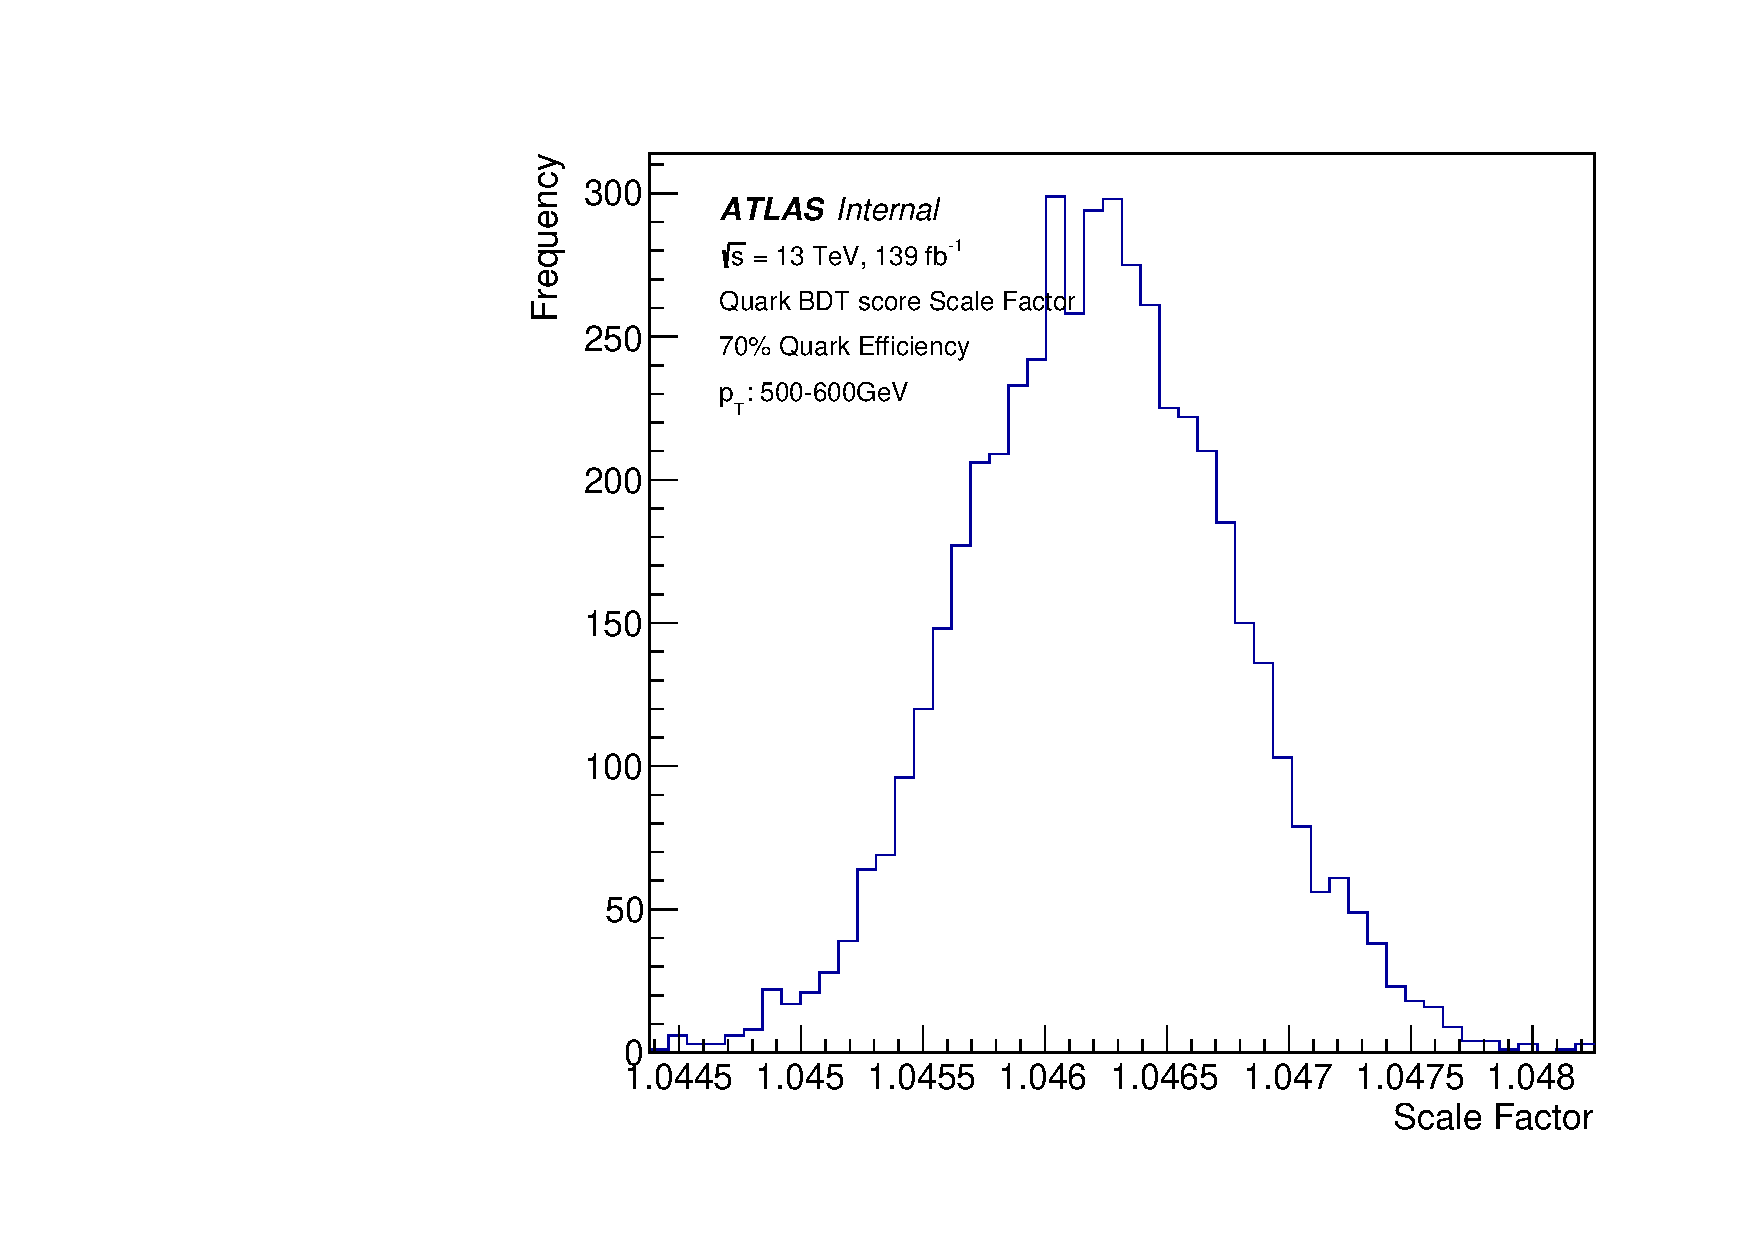
\includegraphics[width=0.22\textwidth]{fig/Method1/pythia/Bootstrap/500-0.7-bdt-quark.pdf}} \quad
	\subfloat[working Point:80\%~(Quark)]{\label{fig:QG-pythia-BDTQ8}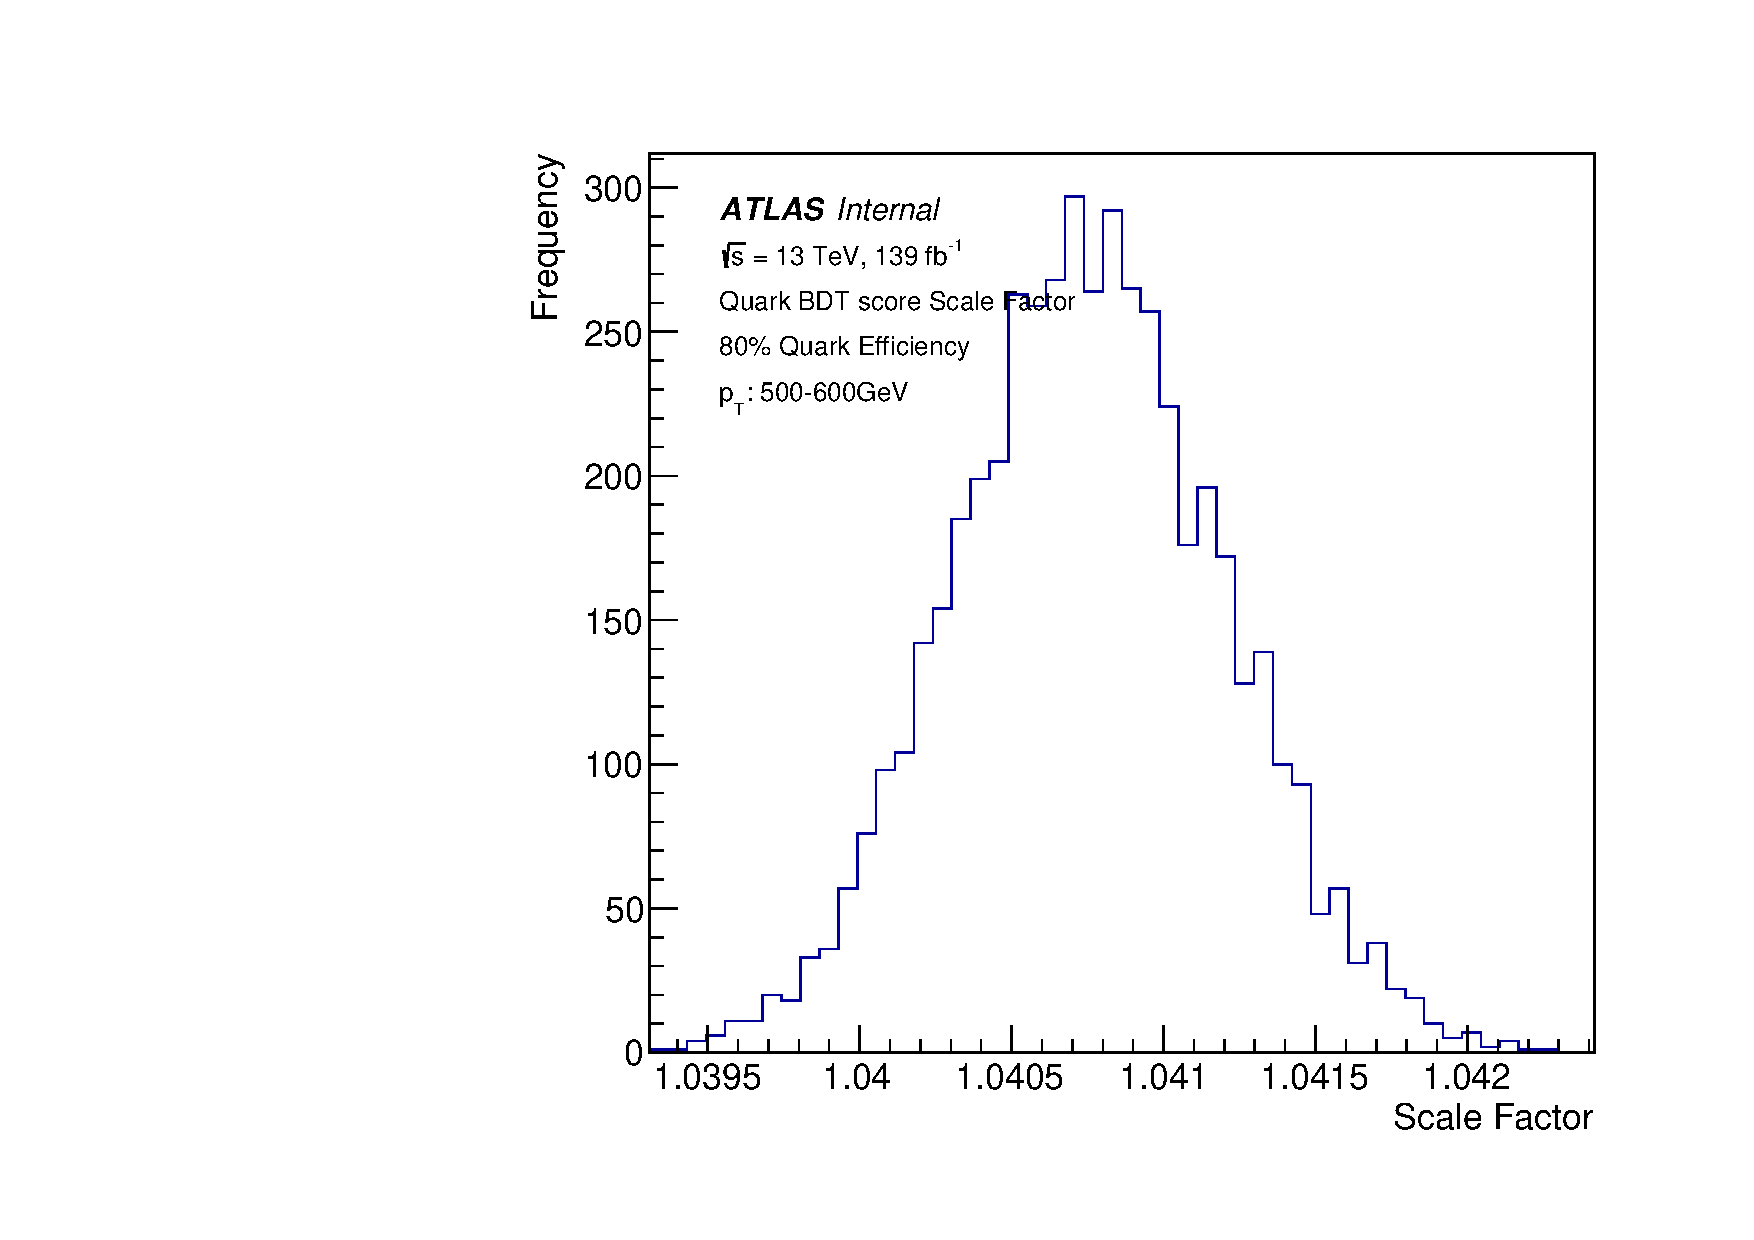
\includegraphics[width=0.22\textwidth]{fig/Method1/pythia/Bootstrap/500-0.8-bdt-quark.pdf}}\\
	\subfloat[working Point:50\%~(Gluon)]{\label{fig:QG-pythia-BDTG5}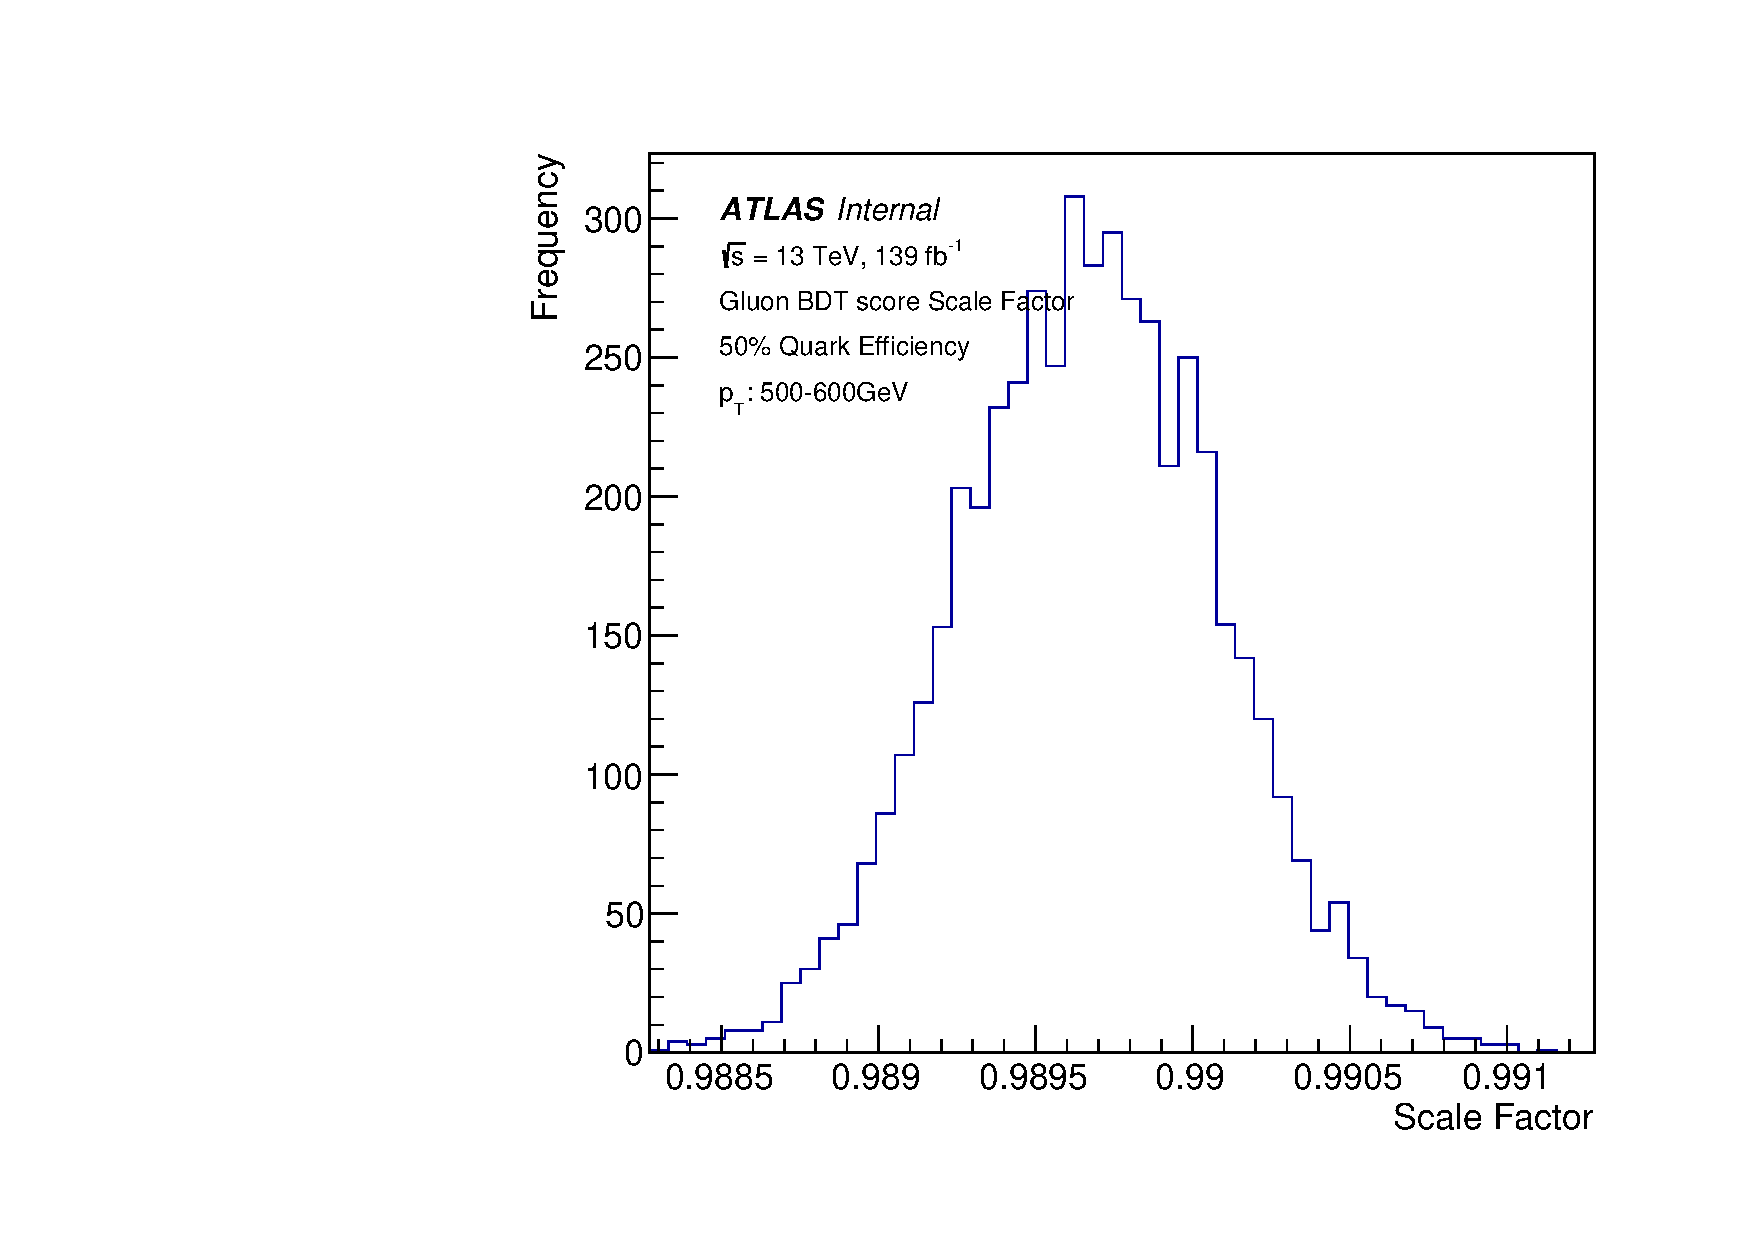
\includegraphics[width=0.22\textwidth]{fig/Method1/pythia/Bootstrap/500-0.5-bdt-gluon.pdf}} \quad
	\subfloat[working Point:60\%~(Gluon)]{\label{fig:QG-pythia-BDTG6}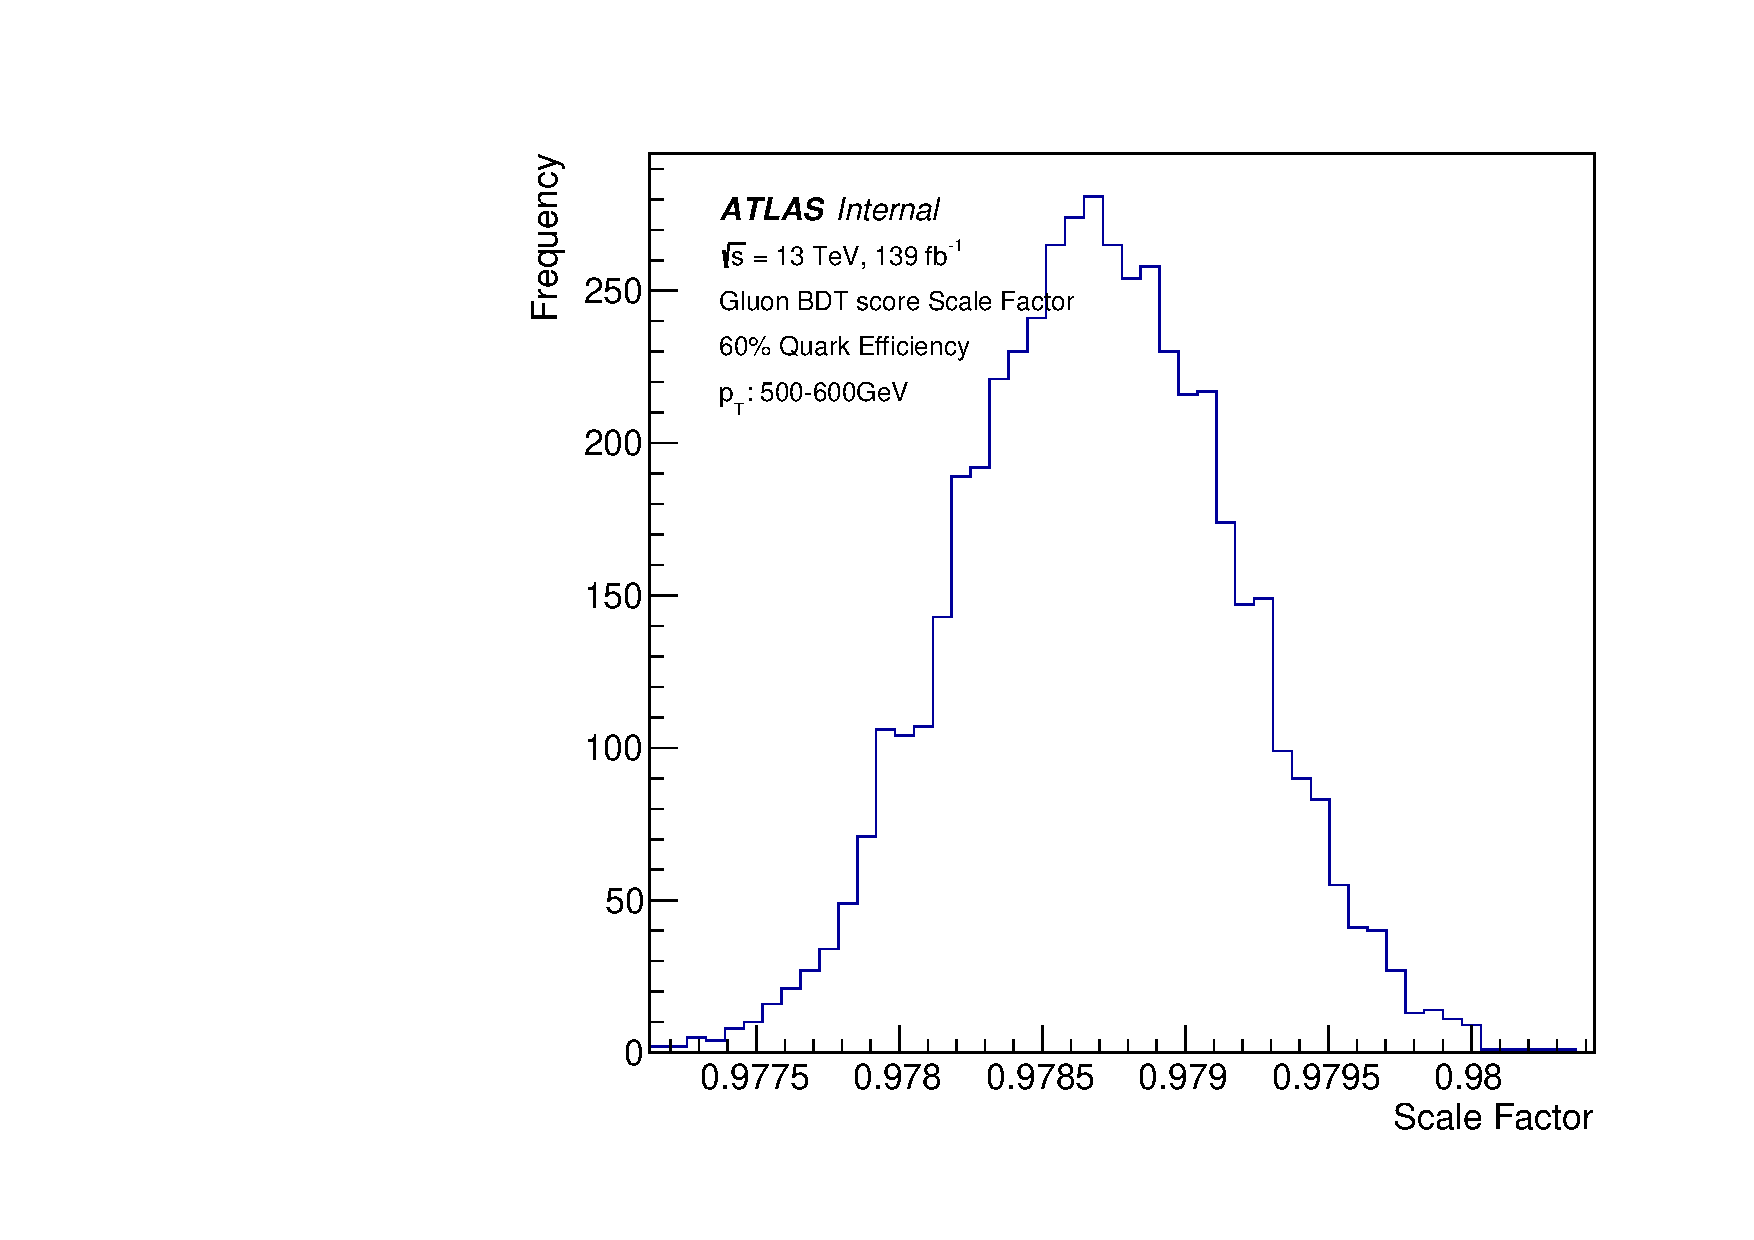
\includegraphics[width=0.22\textwidth]{fig/Method1/pythia/Bootstrap/500-0.6-bdt-gluon.pdf}}\quad
	\subfloat[working Point:70\%~(Gluon)]{\label{fig:QG-pythia-BDTG7}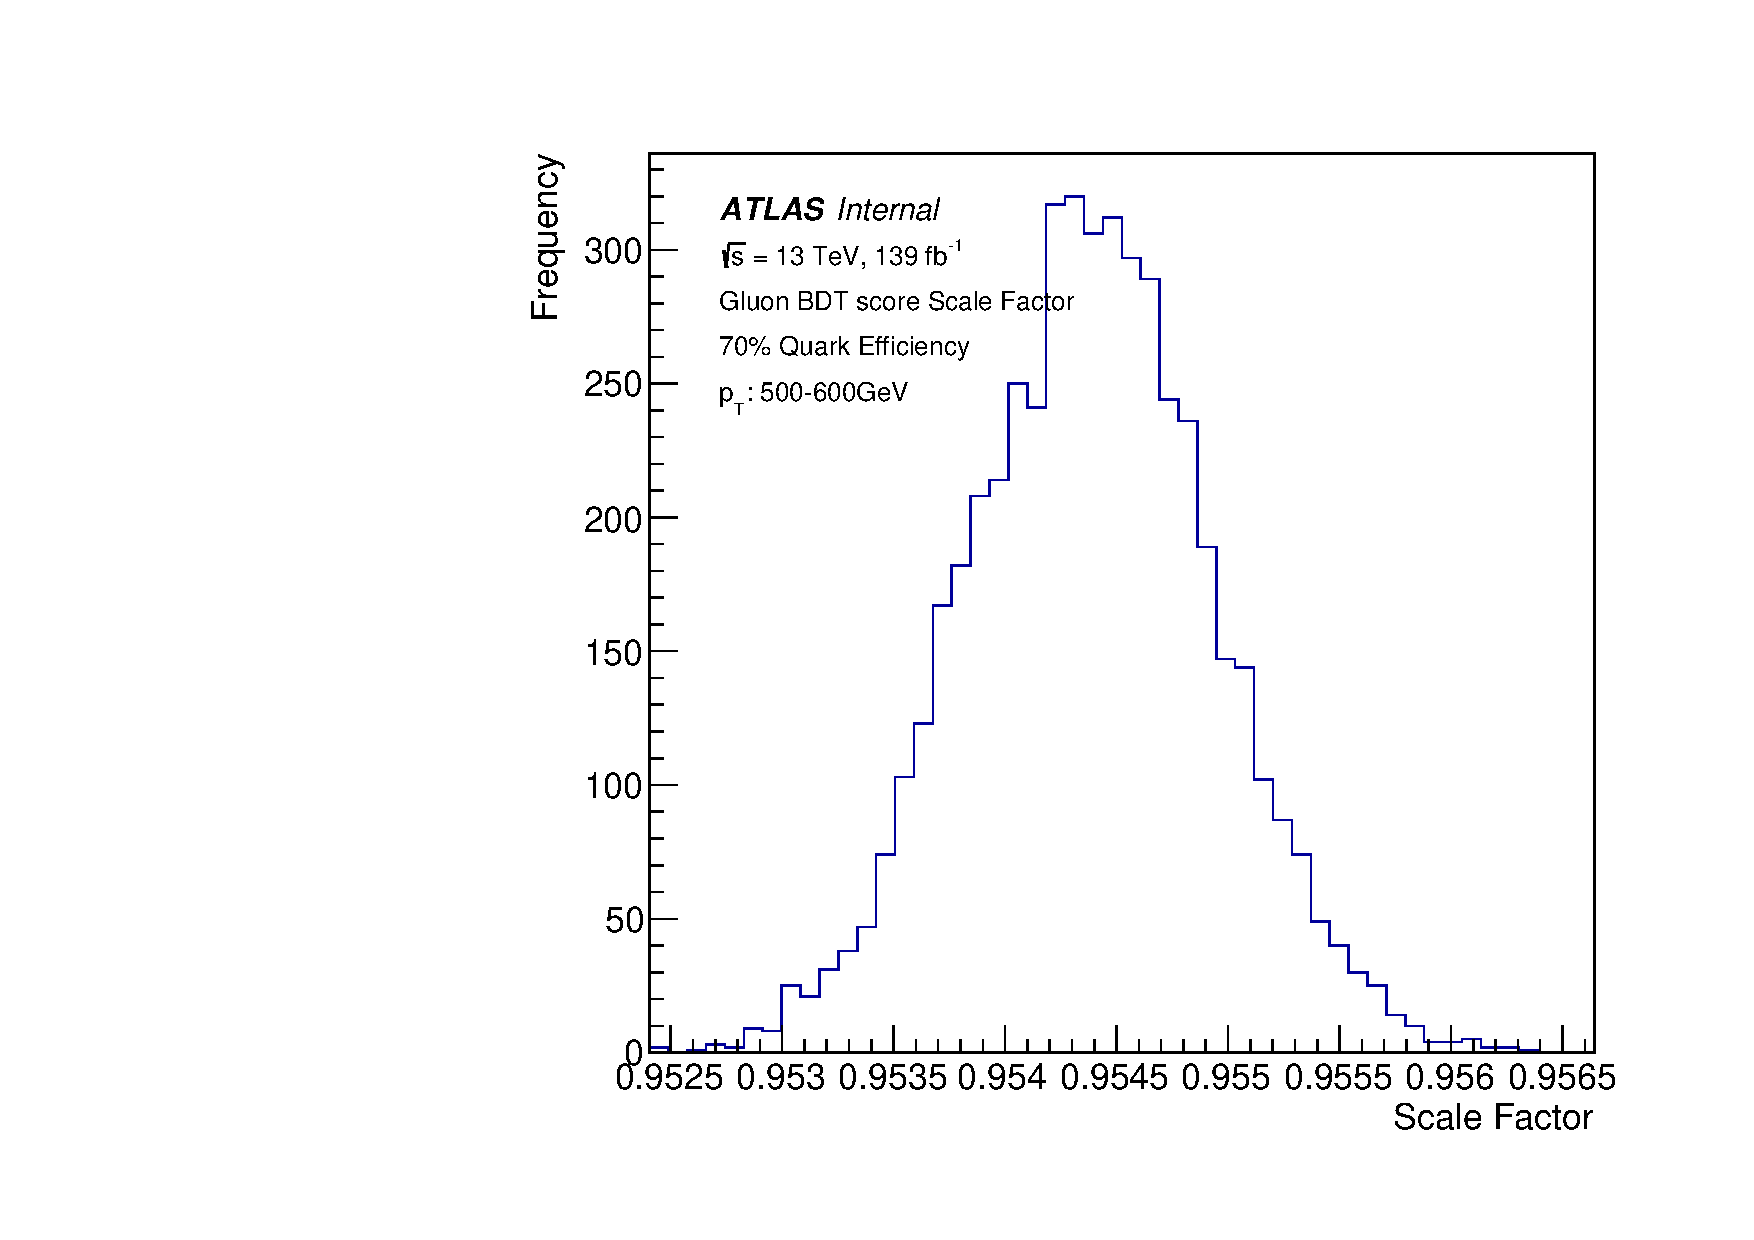
\includegraphics[width=0.22\textwidth]{fig/Method1/pythia/Bootstrap/500-0.7-bdt-gluon.pdf}} \quad
	\subfloat[working Point:80\%~(Gluon)]{\label{fig:QG-pythia-BDTG8}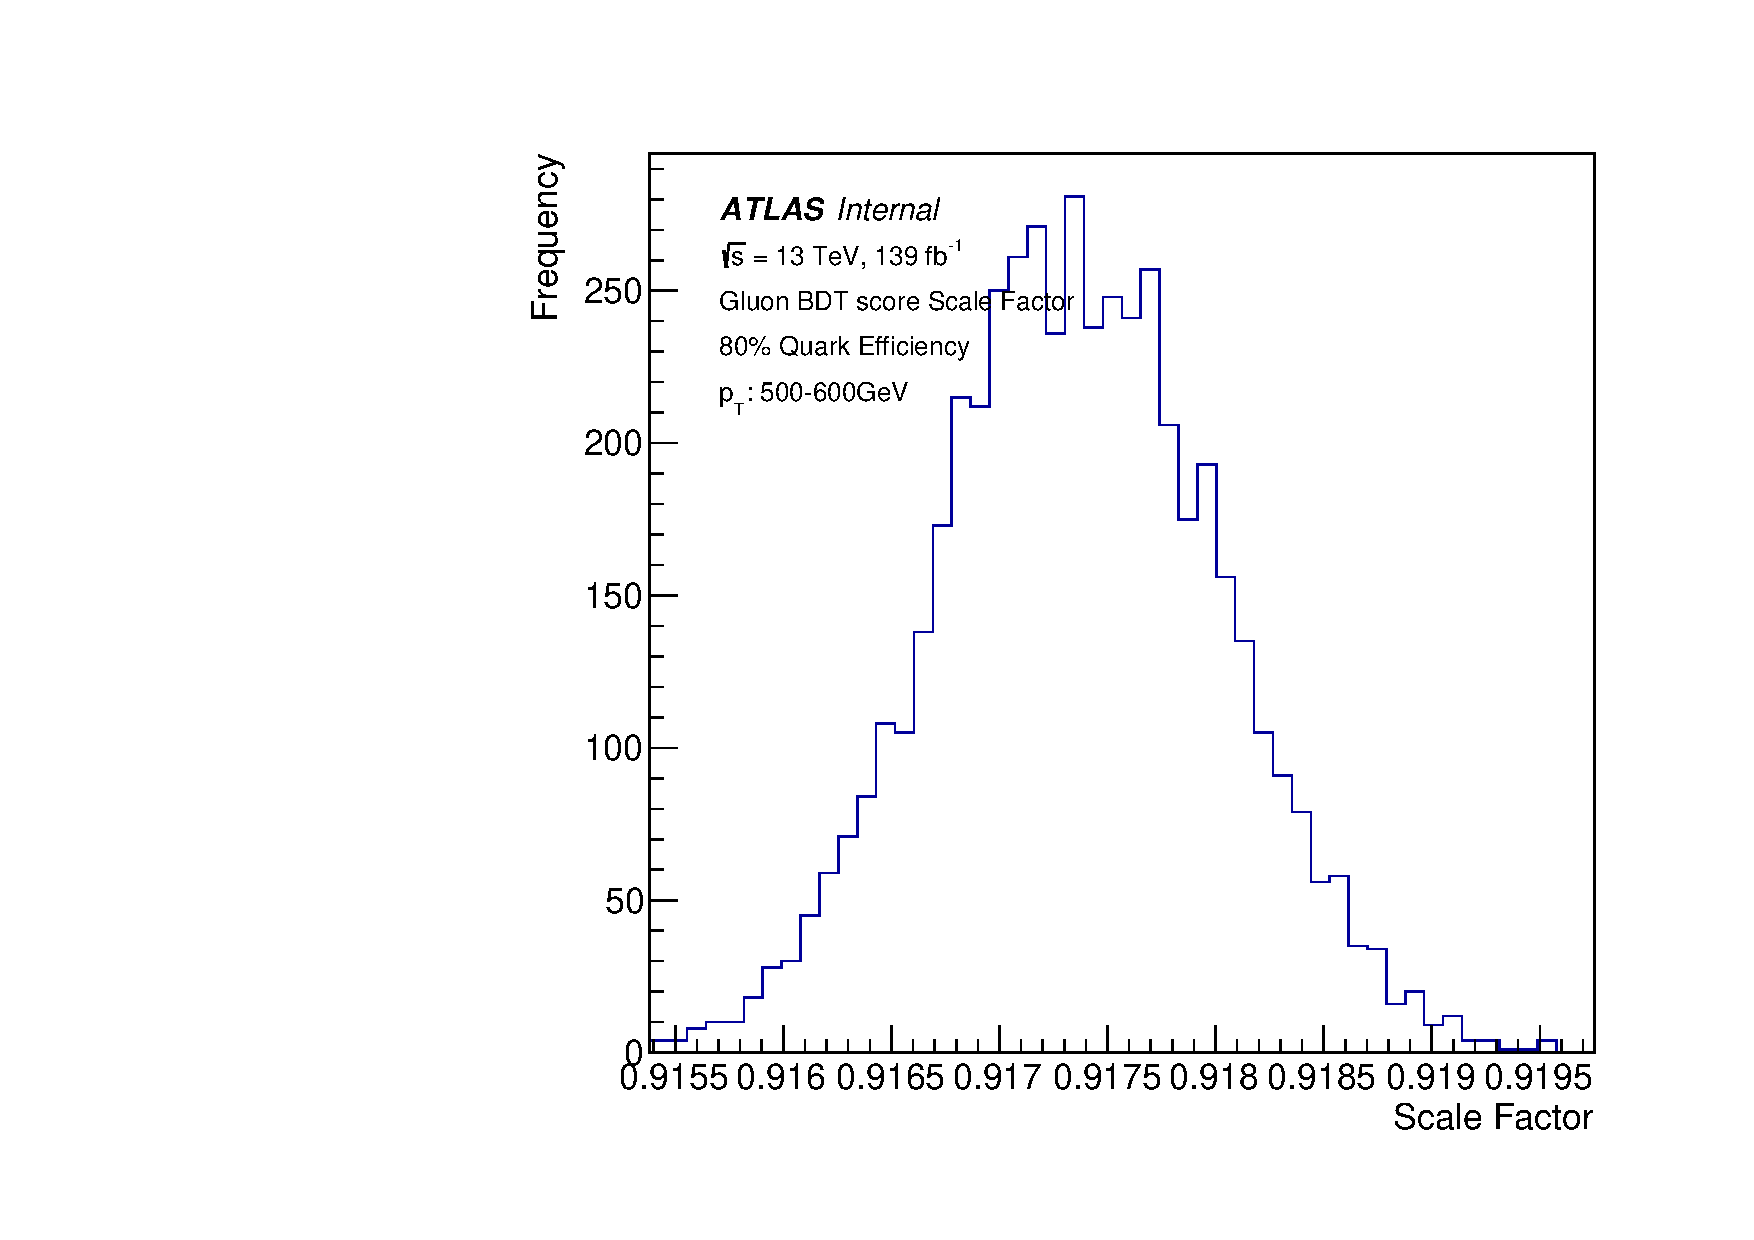
\includegraphics[width=0.22\textwidth]{fig/Method1/pythia/Bootstrap/500-0.8-bdt-gluon.pdf}}\\
	\caption[]{
	The distribution of SF by varying the input data distributions bin-by-bin using a Poisson distribution with the number of data events in each bin as the central value for 5000 times for working point of BDT in jet \pt~range 500-600 GeV. 

		\label{fig:QG-pythia-bootstrap-500-bdt}
	}
\end{figure}






\FloatBarrier

